% Options for packages loaded elsewhere
\PassOptionsToPackage{unicode}{hyperref}
\PassOptionsToPackage{hyphens}{url}
\PassOptionsToPackage{dvipsnames,svgnames,x11names}{xcolor}
%
\documentclass[
  letterpaper,
  DIV=11,
  numbers=noendperiod]{scrreprt}

\usepackage{amsmath,amssymb}
\usepackage{lmodern}
\usepackage{iftex}
\ifPDFTeX
  \usepackage[T1]{fontenc}
  \usepackage[utf8]{inputenc}
  \usepackage{textcomp} % provide euro and other symbols
\else % if luatex or xetex
  \usepackage{unicode-math}
  \defaultfontfeatures{Scale=MatchLowercase}
  \defaultfontfeatures[\rmfamily]{Ligatures=TeX,Scale=1}
\fi
% Use upquote if available, for straight quotes in verbatim environments
\IfFileExists{upquote.sty}{\usepackage{upquote}}{}
\IfFileExists{microtype.sty}{% use microtype if available
  \usepackage[]{microtype}
  \UseMicrotypeSet[protrusion]{basicmath} % disable protrusion for tt fonts
}{}
\makeatletter
\@ifundefined{KOMAClassName}{% if non-KOMA class
  \IfFileExists{parskip.sty}{%
    \usepackage{parskip}
  }{% else
    \setlength{\parindent}{0pt}
    \setlength{\parskip}{6pt plus 2pt minus 1pt}}
}{% if KOMA class
  \KOMAoptions{parskip=half}}
\makeatother
\usepackage{xcolor}
\usepackage[lmargin=2.5cm,rmargin=2cm,tmargin=2cm,bmargin=2cm]{geometry}
\setlength{\emergencystretch}{3em} % prevent overfull lines
\setcounter{secnumdepth}{5}
% Make \paragraph and \subparagraph free-standing
\ifx\paragraph\undefined\else
  \let\oldparagraph\paragraph
  \renewcommand{\paragraph}[1]{\oldparagraph{#1}\mbox{}}
\fi
\ifx\subparagraph\undefined\else
  \let\oldsubparagraph\subparagraph
  \renewcommand{\subparagraph}[1]{\oldsubparagraph{#1}\mbox{}}
\fi

\usepackage{color}
\usepackage{fancyvrb}
\newcommand{\VerbBar}{|}
\newcommand{\VERB}{\Verb[commandchars=\\\{\}]}
\DefineVerbatimEnvironment{Highlighting}{Verbatim}{commandchars=\\\{\}}
% Add ',fontsize=\small' for more characters per line
\usepackage{framed}
\definecolor{shadecolor}{RGB}{241,243,245}
\newenvironment{Shaded}{\begin{snugshade}}{\end{snugshade}}
\newcommand{\AlertTok}[1]{\textcolor[rgb]{0.68,0.00,0.00}{#1}}
\newcommand{\AnnotationTok}[1]{\textcolor[rgb]{0.37,0.37,0.37}{#1}}
\newcommand{\AttributeTok}[1]{\textcolor[rgb]{0.40,0.45,0.13}{#1}}
\newcommand{\BaseNTok}[1]{\textcolor[rgb]{0.68,0.00,0.00}{#1}}
\newcommand{\BuiltInTok}[1]{\textcolor[rgb]{0.00,0.23,0.31}{#1}}
\newcommand{\CharTok}[1]{\textcolor[rgb]{0.13,0.47,0.30}{#1}}
\newcommand{\CommentTok}[1]{\textcolor[rgb]{0.37,0.37,0.37}{#1}}
\newcommand{\CommentVarTok}[1]{\textcolor[rgb]{0.37,0.37,0.37}{\textit{#1}}}
\newcommand{\ConstantTok}[1]{\textcolor[rgb]{0.56,0.35,0.01}{#1}}
\newcommand{\ControlFlowTok}[1]{\textcolor[rgb]{0.00,0.23,0.31}{#1}}
\newcommand{\DataTypeTok}[1]{\textcolor[rgb]{0.68,0.00,0.00}{#1}}
\newcommand{\DecValTok}[1]{\textcolor[rgb]{0.68,0.00,0.00}{#1}}
\newcommand{\DocumentationTok}[1]{\textcolor[rgb]{0.37,0.37,0.37}{\textit{#1}}}
\newcommand{\ErrorTok}[1]{\textcolor[rgb]{0.68,0.00,0.00}{#1}}
\newcommand{\ExtensionTok}[1]{\textcolor[rgb]{0.00,0.23,0.31}{#1}}
\newcommand{\FloatTok}[1]{\textcolor[rgb]{0.68,0.00,0.00}{#1}}
\newcommand{\FunctionTok}[1]{\textcolor[rgb]{0.28,0.35,0.67}{#1}}
\newcommand{\ImportTok}[1]{\textcolor[rgb]{0.00,0.46,0.62}{#1}}
\newcommand{\InformationTok}[1]{\textcolor[rgb]{0.37,0.37,0.37}{#1}}
\newcommand{\KeywordTok}[1]{\textcolor[rgb]{0.00,0.23,0.31}{#1}}
\newcommand{\NormalTok}[1]{\textcolor[rgb]{0.00,0.23,0.31}{#1}}
\newcommand{\OperatorTok}[1]{\textcolor[rgb]{0.37,0.37,0.37}{#1}}
\newcommand{\OtherTok}[1]{\textcolor[rgb]{0.00,0.23,0.31}{#1}}
\newcommand{\PreprocessorTok}[1]{\textcolor[rgb]{0.68,0.00,0.00}{#1}}
\newcommand{\RegionMarkerTok}[1]{\textcolor[rgb]{0.00,0.23,0.31}{#1}}
\newcommand{\SpecialCharTok}[1]{\textcolor[rgb]{0.37,0.37,0.37}{#1}}
\newcommand{\SpecialStringTok}[1]{\textcolor[rgb]{0.13,0.47,0.30}{#1}}
\newcommand{\StringTok}[1]{\textcolor[rgb]{0.13,0.47,0.30}{#1}}
\newcommand{\VariableTok}[1]{\textcolor[rgb]{0.07,0.07,0.07}{#1}}
\newcommand{\VerbatimStringTok}[1]{\textcolor[rgb]{0.13,0.47,0.30}{#1}}
\newcommand{\WarningTok}[1]{\textcolor[rgb]{0.37,0.37,0.37}{\textit{#1}}}

\providecommand{\tightlist}{%
  \setlength{\itemsep}{0pt}\setlength{\parskip}{0pt}}\usepackage{longtable,booktabs,array}
\usepackage{calc} % for calculating minipage widths
% Correct order of tables after \paragraph or \subparagraph
\usepackage{etoolbox}
\makeatletter
\patchcmd\longtable{\par}{\if@noskipsec\mbox{}\fi\par}{}{}
\makeatother
% Allow footnotes in longtable head/foot
\IfFileExists{footnotehyper.sty}{\usepackage{footnotehyper}}{\usepackage{footnote}}
\makesavenoteenv{longtable}
\usepackage{graphicx}
\makeatletter
\def\maxwidth{\ifdim\Gin@nat@width>\linewidth\linewidth\else\Gin@nat@width\fi}
\def\maxheight{\ifdim\Gin@nat@height>\textheight\textheight\else\Gin@nat@height\fi}
\makeatother
% Scale images if necessary, so that they will not overflow the page
% margins by default, and it is still possible to overwrite the defaults
% using explicit options in \includegraphics[width, height, ...]{}
\setkeys{Gin}{width=\maxwidth,height=\maxheight,keepaspectratio}
% Set default figure placement to htbp
\makeatletter
\def\fps@figure{htbp}
\makeatother
\newlength{\cslhangindent}
\setlength{\cslhangindent}{1.5em}
\newlength{\csllabelwidth}
\setlength{\csllabelwidth}{3em}
\newlength{\cslentryspacingunit} % times entry-spacing
\setlength{\cslentryspacingunit}{\parskip}
\newenvironment{CSLReferences}[2] % #1 hanging-ident, #2 entry spacing
 {% don't indent paragraphs
  \setlength{\parindent}{0pt}
  % turn on hanging indent if param 1 is 1
  \ifodd #1
  \let\oldpar\par
  \def\par{\hangindent=\cslhangindent\oldpar}
  \fi
  % set entry spacing
  \setlength{\parskip}{#2\cslentryspacingunit}
 }%
 {}
\usepackage{calc}
\newcommand{\CSLBlock}[1]{#1\hfill\break}
\newcommand{\CSLLeftMargin}[1]{\parbox[t]{\csllabelwidth}{#1}}
\newcommand{\CSLRightInline}[1]{\parbox[t]{\linewidth - \csllabelwidth}{#1}\break}
\newcommand{\CSLIndent}[1]{\hspace{\cslhangindent}#1}

\KOMAoption{captions}{tableheading}
\usepackage{titling}
\setlength{\droptitle}{-4cm}
\pretitle{
  \begin{center}
  
\includegraphics[width=16cm,height=2.54cm]{images/pw_logo.jpg}\\ % cover figure
  \vspace{1cm}
  \normalsize
  Instytut Informatyki \\
  \vspace{1.5cm}
  \Large
  Studia Podyplomowe \\
  Big Data - przetwarzanie i analiza dużych zbiorów danych \\
  \vspace{1.5cm}
  PRACA KOŃCOWA \\
  \vspace{2cm}
  \Large
  Michał Kamiński \\
  \vspace{1cm}
  
}
\posttitle{
  \vspace{3cm}
  \end{center}
  }
\preauthor{\begin{center}}
\postauthor{
  Warszawa, 2023
  \end{center}
  \newpage
  \Large 
  \textbf{Streszczenie} \\ \\
  \normalsize
  W niniejszej pracy zaprezentowano przykładową infrastrukturę wykorzystującą zasoby chmury 
  AWS (ang. \emph{Amazon Web Services}) umożliwiającą analizę dużych zbiorów danych za pomocą klastów 
  obliczeniowych przy użyciu serwisu AWS EMR (ang. \emph{Elastic Map Reduce}). Zaprezentowano, jak 
  przygotować przykładowe dane oraz dokonano wstępnej analizy danych pochodzących z repozytorium 
  Stack Exchange przy użyciu technologii Spark, wykorzystując API w języku Python (pySpark) \\
  
  Słowa kluczowe: \textbf{Big Data, Spark, AWS, EMR, S3} \\ \\ \\ 

  \hrulefill

  \Large 
  \textbf{Summary} \\ \\
  \normalsize
  The thesis demonstrates the cloud infrastructure built using Amazon Web Services (AWS), that 
  allows efficient analysis of large data sets (Big Data) using distributed computing system with 
  example of AWS Elastic Map Reduce (EMR) service. As a demonstration of data preparation and initial 
  analysis, python Spark API (pySpark) was used to analyze data from one of Stack Exchange forum. \\

  Keywords: \textbf{Big Data, Spark, AWS, EMR, S3} \\
}
\makeatletter
\makeatother
\makeatletter
\@ifpackageloaded{bookmark}{}{\usepackage{bookmark}}
\makeatother
\makeatletter
\@ifpackageloaded{caption}{}{\usepackage{caption}}
\AtBeginDocument{%
\ifdefined\contentsname
  \renewcommand*\contentsname{Spis treści}
\else
  \newcommand\contentsname{Spis treści}
\fi
\ifdefined\listfigurename
  \renewcommand*\listfigurename{Spis rycin}
\else
  \newcommand\listfigurename{Spis rycin}
\fi
\ifdefined\listtablename
  \renewcommand*\listtablename{Spis tabel}
\else
  \newcommand\listtablename{Spis tabel}
\fi
\ifdefined\figurename
  \renewcommand*\figurename{Rysunek}
\else
  \newcommand\figurename{Rysunek}
\fi
\ifdefined\tablename
  \renewcommand*\tablename{Tabela}
\else
  \newcommand\tablename{Tabela}
\fi
}
\@ifpackageloaded{float}{}{\usepackage{float}}
\floatstyle{ruled}
\@ifundefined{c@chapter}{\newfloat{codelisting}{h}{lop}}{\newfloat{codelisting}{h}{lop}[chapter]}
\floatname{codelisting}{Wykaz}
\newcommand*\listoflistings{\listof{codelisting}{Spis wykazów}}
\makeatother
\makeatletter
\@ifpackageloaded{caption}{}{\usepackage{caption}}
\@ifpackageloaded{subcaption}{}{\usepackage{subcaption}}
\makeatother
\makeatletter
\@ifpackageloaded{tcolorbox}{}{\usepackage[many]{tcolorbox}}
\makeatother
\makeatletter
\@ifundefined{shadecolor}{\definecolor{shadecolor}{rgb}{.97, .97, .97}}
\makeatother
\makeatletter
\makeatother
\ifLuaTeX
\usepackage[bidi=basic]{babel}
\else
\usepackage[bidi=default]{babel}
\fi
\babelprovide[main,import]{polish}
% get rid of language-specific shorthands (see #6817):
\let\LanguageShortHands\languageshorthands
\def\languageshorthands#1{}
\ifLuaTeX
  \usepackage{selnolig}  % disable illegal ligatures
\fi
\usepackage[]{biblatex}
\addbibresource{references.bib}
\IfFileExists{bookmark.sty}{\usepackage{bookmark}}{\usepackage{hyperref}}
\IfFileExists{xurl.sty}{\usepackage{xurl}}{} % add URL line breaks if available
\urlstyle{same} % disable monospaced font for URLs
\hypersetup{
  pdftitle={Wieloskalowa analiza danych z forum internetowego przy użyciu usług chmury AWS},
  pdflang={pl},
  colorlinks=true,
  linkcolor={blue},
  filecolor={Maroon},
  citecolor={Blue},
  urlcolor={Blue},
  pdfcreator={LaTeX via pandoc}}

\title{Wieloskalowa analiza danych z forum internetowego przy użyciu
usług chmury AWS}
\author{}
\date{}

\begin{document}
\maketitle
\ifdefined\Shaded\renewenvironment{Shaded}{\begin{tcolorbox}[frame hidden, borderline west={3pt}{0pt}{shadecolor}, boxrule=0pt, interior hidden, breakable, enhanced, sharp corners]}{\end{tcolorbox}}\fi

\renewcommand*\contentsname{Spis treści}
{
\hypersetup{linkcolor=}
\setcounter{tocdepth}{2}
\tableofcontents
}
\bookmarksetup{startatroot}

\hypertarget{streszczenie}{%
\chapter*{Streszczenie}\label{streszczenie}}
\addcontentsline{toc}{chapter}{Streszczenie}

\markboth{Streszczenie}{Streszczenie}

W niniejszej pracy zaprezentowano przykładową infrastrukturę
wykorzystującą zasoby chmury AWS (ang. \emph{Amazon Web Services})
umożliwiającą analizę dużych zbiorów danych za pomocą klastów
obliczeniowych przy użyciu serwisu AWS EMR (ang. \emph{Elastic Map
Reduce}). Zaprezentowano, jak przygotować przykładowe dane oraz dokonano
wstępnej analizy danych pochodzących z repozytorium Stack Exchange przy
użyciu technologii Spark, wykorzystując API w języku Python (pySpark)

Słowa kluczowe: Big Data, Spark, AWS, EMR, S3

\hypertarget{summary}{%
\section*{Summary}\label{summary}}
\addcontentsline{toc}{section}{Summary}

\markright{Summary}

The thesis demonstrates the cloud infrastructure built using Amazon Web
Services (AWS), that allows efficient analysis of large data sets (Big
Data) using distributed computing system with example of AWS Elastic Map
Reduce (EMR) service. As a demonstration of data preparation and initial
analysis, python Spark API (pySpark) was used to analyze data from one
of Stack Exchange forum.

Keywords: Big Data, Spark, AWS, EMR, S3

\part{Wstęp}

\hypertarget{technologie-big-data}{%
\section*{Technologie big data}\label{technologie-big-data}}
\addcontentsline{toc}{section}{Technologie big data}

\markright{Technologie big data}

Ilość przetwarzanych danych cyfrowych na świecie rośnie w tempie
logarytmicznym i obecnie podawana jest w dziesiątkach zettabajtów
\autocite{bartley_2022}. Wraz ze wzrostem ilości danych niezbędne jest
optymalizowanie bądź zwiększanie miejsca potrzebnego na ich
przechowywanie oraz ulepszanie algorytmów pozwalających na dokonanie
analiz w czasie umożliwiającym na wyciąganie wniosków i podejmowania
stosownych akcji.

Znaczącym usprawnieniem procesu analitycznego było opracowanie algorytmu
\texttt{MapReduce} \autocite{dean_ghhemawat_2010}, wykorzystującego
równoległe przetwarzanie zbiorów danych w klastrach komputerowych.
Opiera się na stosowaniu dwóch ``kroków''. Kroku \texttt{map}
odpowiadającego za wykonaywanie zadań w węzłach roboczych (niezależnie
od siebie) a następnie kroku \texttt{reduce}, który zbiera dane z węzłów
roboczych i dokonuje kroku redukcji danych poprzez np. agregację.

Klastry komputerowe mogą być wykorzystywane nie tylko do obliczeń, ale
również do przechowywania danych. Platformą, która wykorzystuje
rozproszony system plików jest np. \texttt{Apache\ Hadoop} i sytem HDFS
\autocite{apache_hadoop}. System HDFS daje możliwość na zwiększenie
dostępności danych poprzez ich replikację. W przypadku niedostępności
jednego z węzłów roboczych, dane są dostępne na pozostałych węzłach.
Dodatkowo poprzez odpowiednie partycjonowanie danych można usprawnić
działania analityczne, które ograniczą wysyłanie danych po sieci klastra
\autocite{navarro_2017}.

\texttt{Apache\ Hadoop} i \texttt{MapReduce} mają jednak swoje
ograniczenia, z czego jednym z bardziej znaczących jest konieczność
wczytywania danych z dysku dla każdego zadania, co jest mało wydajne
przy zadaniach wykonywanych w sposób iteracyjny jak np. trenowanie
modeli statystycznych z wieloma hiperparametrami \autocite{spark_2010}.
W pracy \textcite{spark_2010}, zaprezentowano techologię \texttt{Spark}
(obecnie \texttt{Apache\ Spark}), która obchodzi te ograniczenia poprzez
wykorzystanie pamięci RAM oraz wprowadzenie obiektów RDD (ang.
\emph{Resilient Distributed Datasets}) \autocite{rdd_2012}. RDD są
obiektami niemodyfikowalnymi (ang. \emph{immutable}), rozproszonymi po
klastrze i co najistotniejsze przechowywane w pamięci RAM. Dzieki temu
mogą być wykorzystywane wielokrotnie bez konieczności wykonywania
operacji odczytu z dysku, który znacząco obniża tempo wykonywania
obliczeń. Autorzy \textcite{spark_2010} szacują że
\texttt{Apache\ Spark} jest około 10 razy szybszy niż
\texttt{Apache\ Hadoop} w wykonywaniu iteracyjnym operacji związanych z
uczeniem maszynowym.

\hypertarget{formaty-danych}{%
\section*{Formaty danych}\label{formaty-danych}}
\addcontentsline{toc}{section}{Formaty danych}

\markright{Formaty danych}

W czasach sprzed tzw. ery Big Data, dane przechowywane były (oraz często
dalej są) w relacyjnych bazach danych. W najprostszym założeniu
(pomijając możliwości indeksowania oraz stosowania kluczy) dane
przetrzymywane są w klasycznym schemacie, jedna obserwacja - jeden
wiersz, jedna cecha jedna kolumna (zobacz Tabela~\ref{tbl-logical}). W
jaki sposób te dane są przechowywane na dysku obrazuje za to
Rysunek~\ref{fig-row}. Przechowywanie informacji w ten sposób powoduje,
że aby dokonać agregacji cechy znajdującej się w kolumnie o nazwie
\texttt{kolumna1}, algorytm musi przeskanować wszystkie wiersze
wczytując je do pamięci.

Rozwiązaniem, które usprawnia ten proces i wykorzystywane jest w
rozwiązaniach typu Big Data jest przechowywanie danych w sposób
kolumnowy, zaprezentowany na Rysunek~\ref{fig-col}. W tym przypadku
jeżeli naszym celem jest jedynie zagregowanie cechy \texttt{kolumna1} to
tylko dane z tej kolumny zostaną wczytanie do pamięci, ponieważ algorytm
wie, w kórym miejscu na dysku znajdują się dane z tej kolumny.
Przykładem formatów kolumnowych w systemie \texttt{Apache\ Hadoop} są
\texttt{RCFile} oraz \texttt{ORC} a dodatkowo bardzo popularnym formatem
jest format \texttt{Apache\ Parquet}.

Dodatkową zaletą formatów kolumnowych jest kompresja danych i
zwiększenie szybkości wykonywania zapytań Tabela~\ref{tbl-parquet}.

\hypertarget{tbl-logical}{}
\begin{longtable}[]{@{}cccc@{}}
\caption{\label{tbl-logical}Zobrazowanie tabeli rozrysowanej na
Rysunek~\ref{fig-row} oraz Rysunek~\ref{fig-col}}\tabularnewline
\toprule()
& kolumna1 & kolumna2 & kolumna3 \\
\midrule()
\endfirsthead
\toprule()
& kolumna1 & kolumna2 & kolumna3 \\
\midrule()
\endhead
wiersz1 & A & B & C \\
wiersz2 & D & E & F \\
wiersz3 & G & H & I \\
wiersz4 & J & K & L \\
\bottomrule()
\end{longtable}

\begin{figure}

{\centering 

\begin{figure}[H]

{\centering 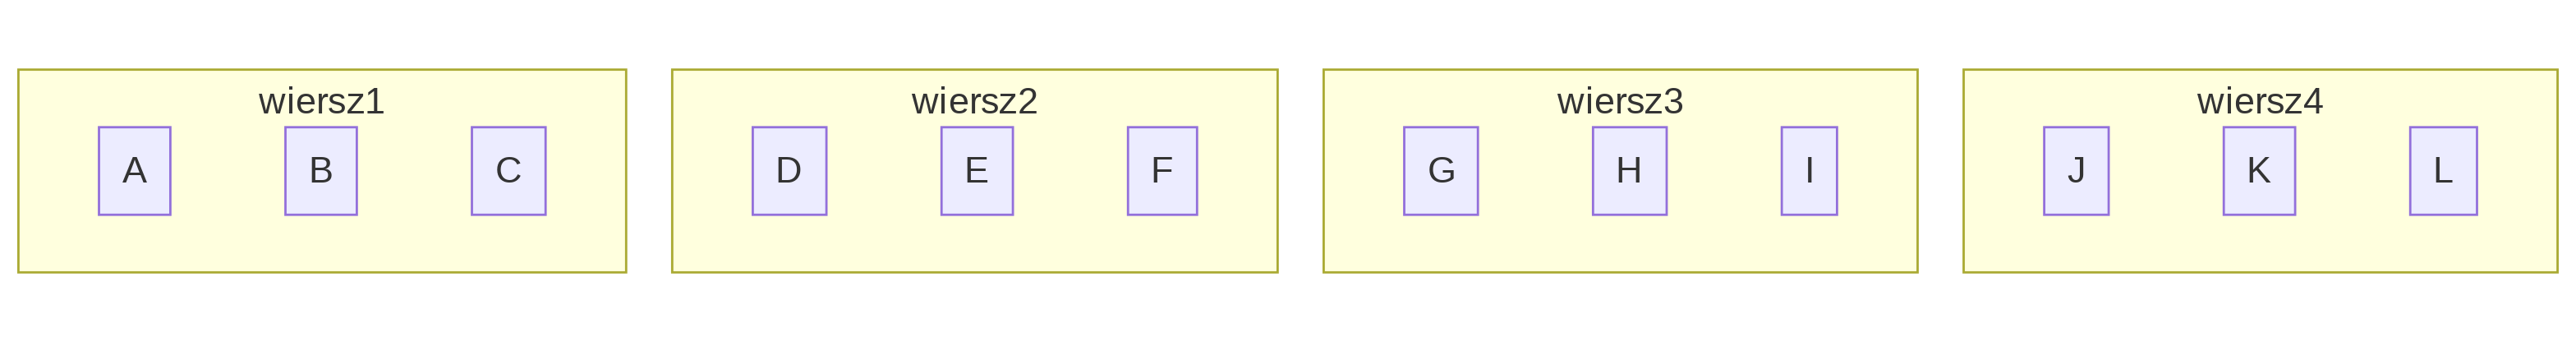
\includegraphics[width=9.5in,height=0.88in]{./intro_files/figure-latex/mermaid-figure-1.png}

}

\end{figure}

}

\caption{\label{fig-row}Przykład wierszowego formatu danych. Kolejność
wierszy przedstawia pozycję na dysku.}

\end{figure}

\begin{figure}

{\centering 

\begin{figure}[H]

{\centering 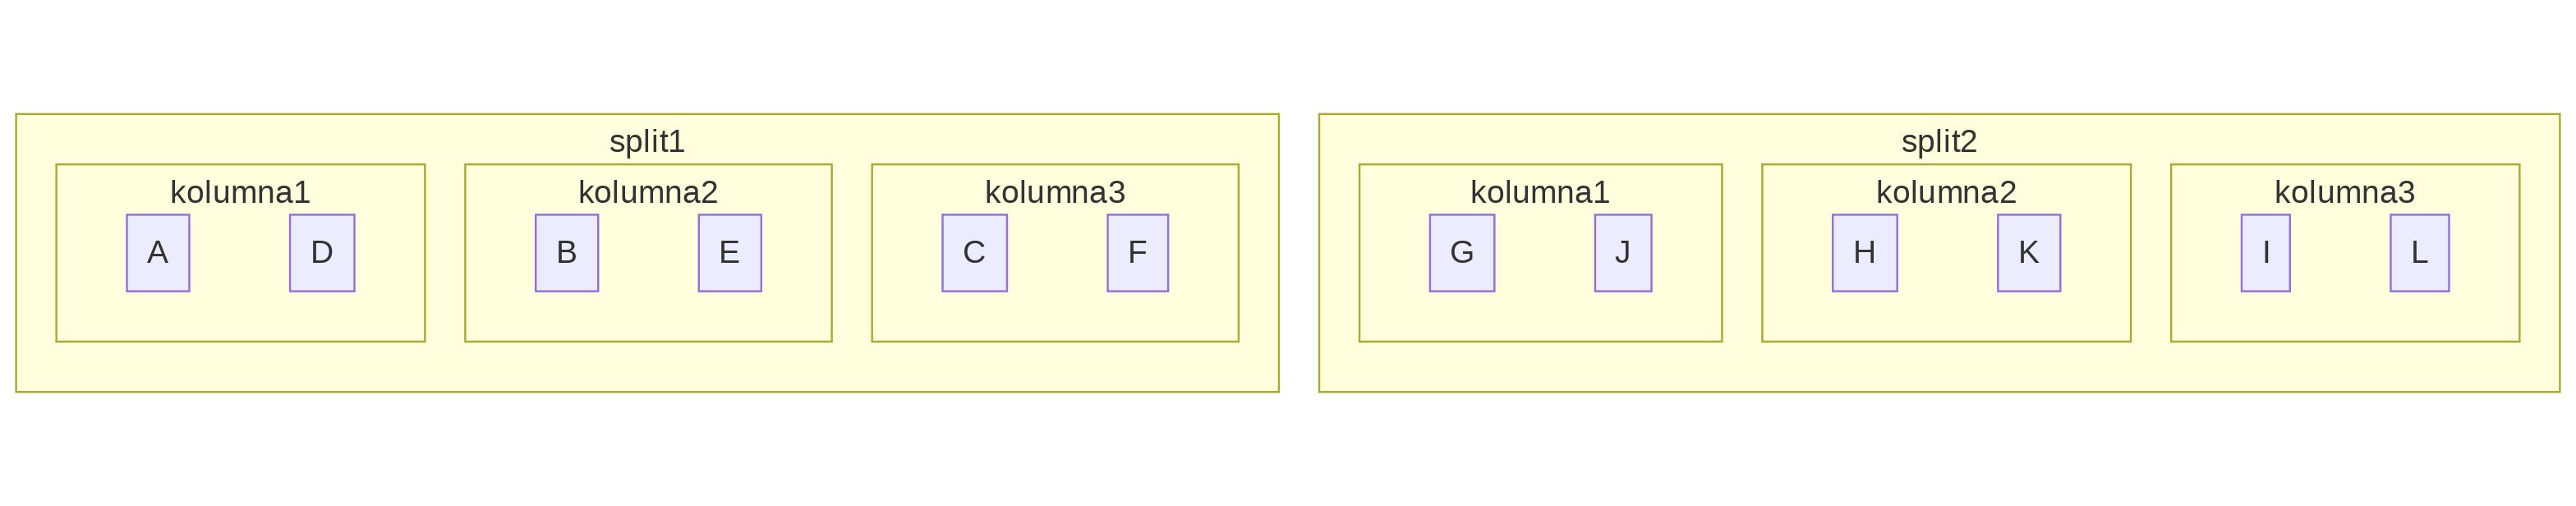
\includegraphics[width=11in,height=1.32in]{./intro_files/figure-latex/mermaid-figure-2.png}

}

\end{figure}

}

\caption{\label{fig-col}Przykład columnowego formatu danych. Kolejność
wierszy przedstawia pozycję na dysku.}

\end{figure}

\hypertarget{tbl-parquet}{}
\begin{longtable}[]{@{}
  >{\raggedright\arraybackslash}p{(\columnwidth - 8\tabcolsep) * \real{0.1720}}
  >{\raggedright\arraybackslash}p{(\columnwidth - 8\tabcolsep) * \real{0.1720}}
  >{\raggedright\arraybackslash}p{(\columnwidth - 8\tabcolsep) * \real{0.3226}}
  >{\raggedright\arraybackslash}p{(\columnwidth - 8\tabcolsep) * \real{0.2581}}
  >{\raggedright\arraybackslash}p{(\columnwidth - 8\tabcolsep) * \real{0.0753}}@{}}
\caption{\label{tbl-parquet}Porównanie formatu CSV z Apache
Parquet}\tabularnewline
\toprule()
\begin{minipage}[b]{\linewidth}\raggedright
Format
\end{minipage} & \begin{minipage}[b]{\linewidth}\raggedright
Rozmiar danych
\end{minipage} & \begin{minipage}[b]{\linewidth}\raggedright
Czas wykonania zapytania (s)
\end{minipage} & \begin{minipage}[b]{\linewidth}\raggedright
Ilość wczytanych danch
\end{minipage} & \begin{minipage}[b]{\linewidth}\raggedright
Koszt (\$)\footnote{Koszt w serwisie AWS S3}
\end{minipage} \\
\midrule()
\endfirsthead
\toprule()
\begin{minipage}[b]{\linewidth}\raggedright
Format
\end{minipage} & \begin{minipage}[b]{\linewidth}\raggedright
Rozmiar danych
\end{minipage} & \begin{minipage}[b]{\linewidth}\raggedright
Czas wykonania zapytania (s)
\end{minipage} & \begin{minipage}[b]{\linewidth}\raggedright
Ilość wczytanych danch
\end{minipage} & \begin{minipage}[b]{\linewidth}\raggedright
Koszt (\$){}
\end{minipage} \\
\midrule()
\endhead
CSV & 1 TB & 236 & 1.15 TB & 5.75 \\
Apache Parquet & 130 GB & 6.78 seconds & 2.51 GB & 0.01 \\
\bottomrule()
\end{longtable}

\hypertarget{chmury}{%
\section*{Chmury}\label{chmury}}
\addcontentsline{toc}{section}{Chmury}

\markright{Chmury}

\hypertarget{cel-pracy}{%
\section*{Cel pracy}\label{cel-pracy}}
\addcontentsline{toc}{section}{Cel pracy}

\markright{Cel pracy}

Celem niniejszej pracy jest utworzenie infrastruktury w chmurze
obliczeniowej AWS pozwalające na wielkoskalową analizy danych w sytemie
rozproszonym (ang. \emph{Big Data}).

Do stworzenia przykładowego projektu wykorzystano dane ze strony
\href{https://stackexchange.com/}{\emph{Stack Exchange}} zawierającej
zestawy danych pochodzące z forów społecznościoowych. Analizę
ograniczono do danych pochodzących z forum o nazwie
\href{https://data.stackexchange.com/beer/queries}{\emph{Beer, Wine and
Spirits}}.

\begin{verbatim}
# header-includes: |
#   \usepackage{titling}

#   \preauthor{
#     \begin{center}
#     
\includegraphics[width=16cm,height=2.54cm]{images/pw_logo.jpg}\\ % cover figure
#     \Large
#   }
#   \postauthor{
#     \end{center}
#   }
#   \predate{
#     \begin{center}
#     Master of Science in Biology\\               % Degree
#     Biodiversity, Evolution and Ecology\\        % Degree stream
#     Department of Biological Sciences\\          % Department
#     University of Bergen\\                       % University 
#     \vspace{5mm}
#   }
#   \postdate{
#     \end{center}
#    }
\end{verbatim}

\part{Wyniki i Dyskusja}

\hypertarget{schemat-infrastruktury}{%
\chapter{Schemat infrastruktury}\label{schemat-infrastruktury}}

\begin{verbatim}
Warning: node '96a5af8ac08745bbb36feba15ffa4f1f', graph '%3' size too small for label
Warning: node '90c5130ba2074f8aac5b6ed48303080e', graph '%3' size too small for label
Warning: node 'e92f82b8ae1b4965bc3679f3f28ffb30', graph '%3' size too small for label
Warning: Orthogonal edges do not currently handle edge labels. Try using xlabels.
\end{verbatim}

\begin{figure}

{\centering 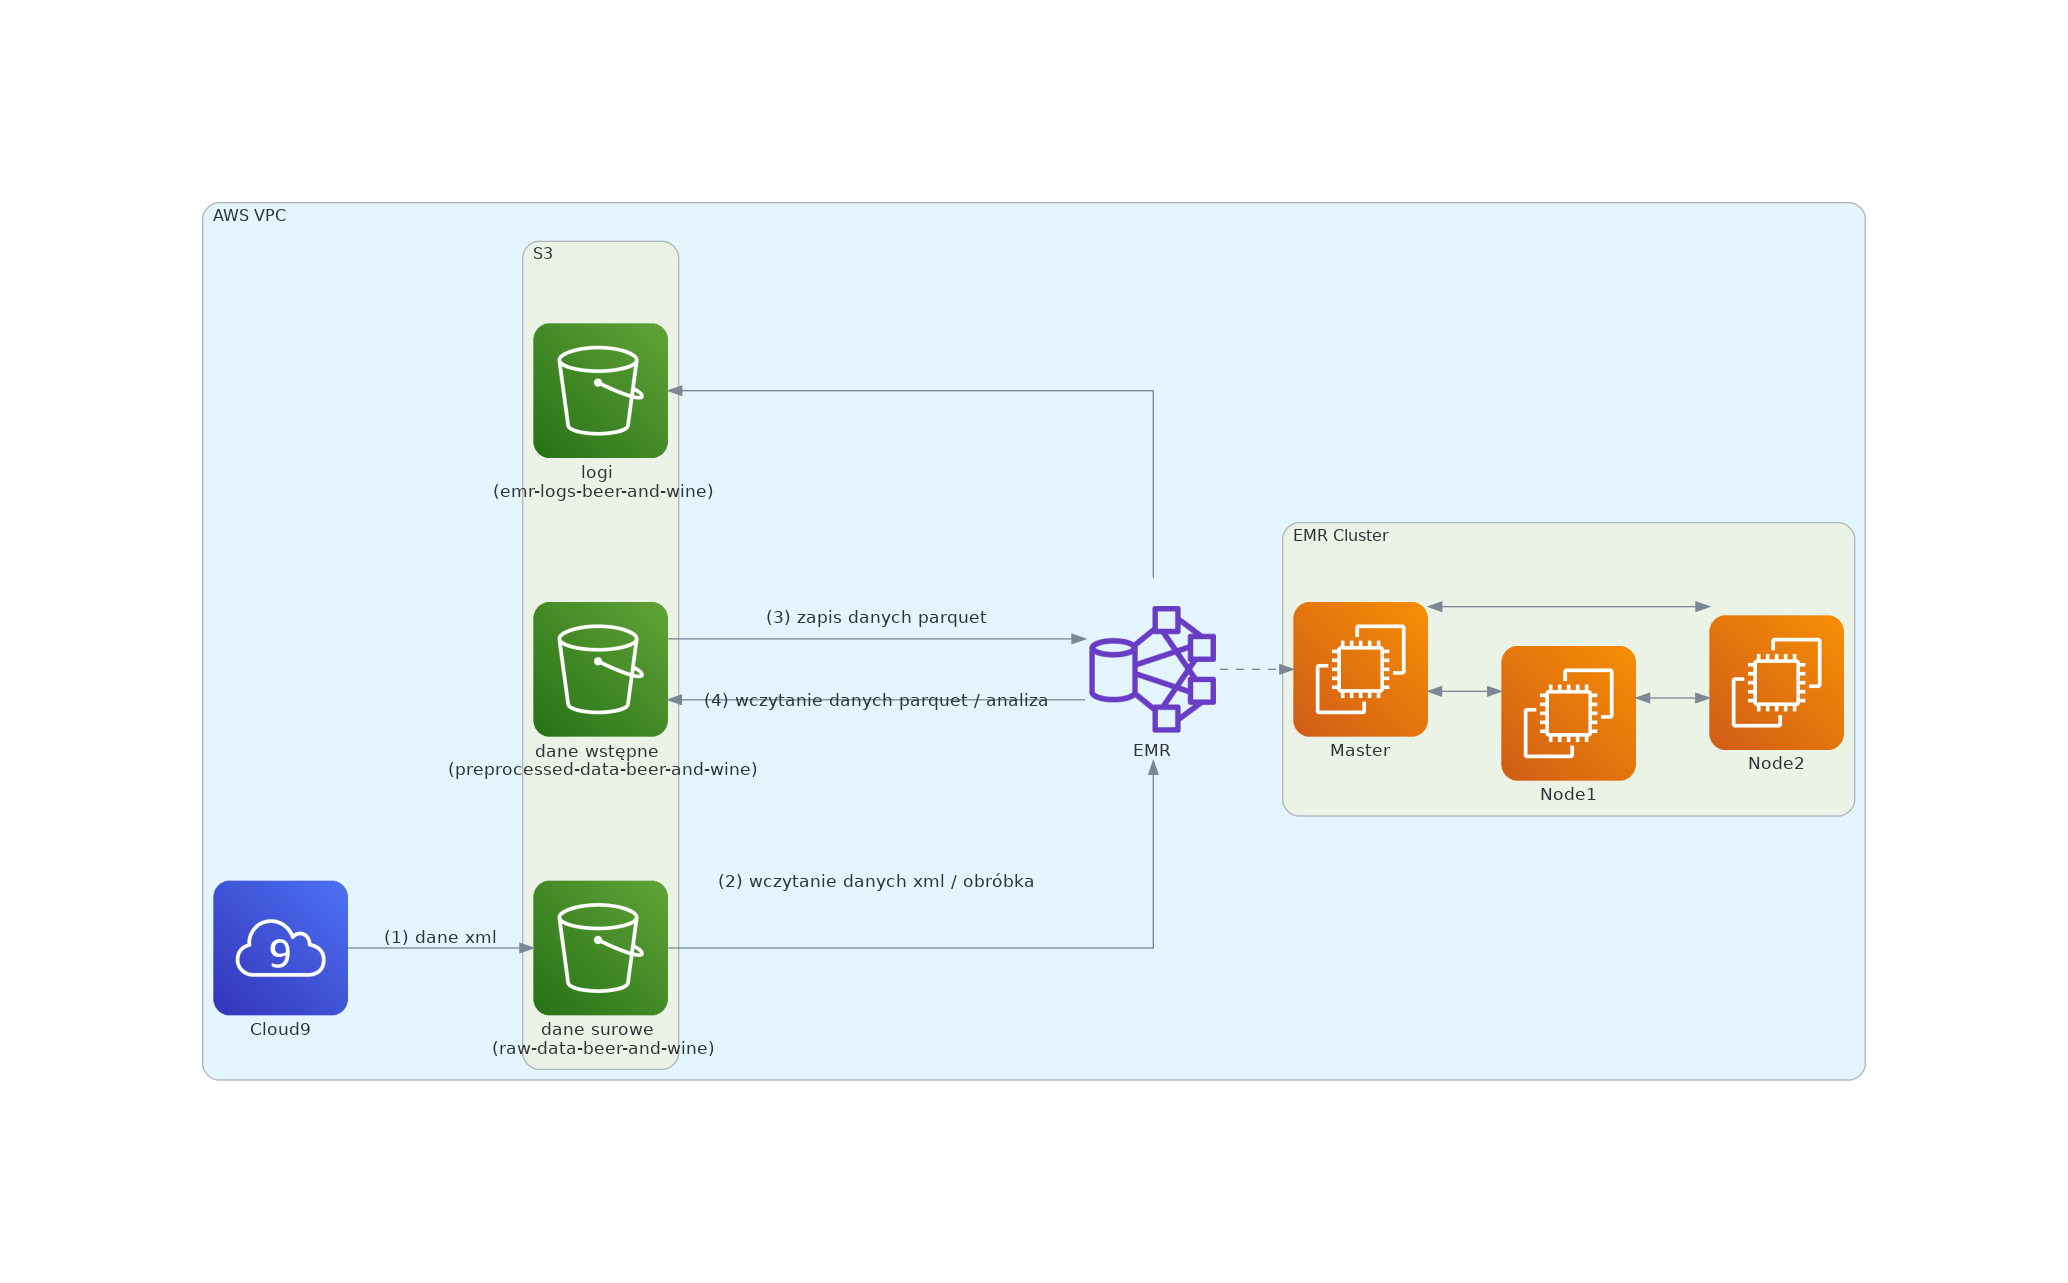
\includegraphics{./00_schema_files/figure-pdf/fig-ryc1-output-2.png}

}

\caption{\label{fig-ryc1}Schemat rozwiązania}

\end{figure}

W celu rozwiązania postawionego problemu analitycznego stworzono
infrastrukturę wyłącznie w obrębie chmury AWS, której ogólny schemat
przedstawiono na Rysunek~\ref{fig-ryc1}

\hypertarget{ekstrakcja}{%
\section{Ekstrakcja}\label{ekstrakcja}}

Do etapu ekstrakcji danych wykorzystano usługę \texttt{Cloud9}, która
zapewnia dostęp do terminala maszyny wirtualnej z systemem linux
(platforma \texttt{Amazon\ Linux\ 2}, typ instancji \texttt{t2.micro}).
Z użyciem tej usługi dane zostały pobrane ze źródła w binarnym formacie
\texttt{7z} a następnie pliki zostały wyekstrahowane w formacie
\texttt{xml} przy pomocy programu \texttt{p7zip}. Dane w formacie
\texttt{xml} zostały następnie skopiowane do serwisu \texttt{S3}, gdzie
utworzono koszyk danych (ang. \emph{bucket}) o nazwie
\texttt{raw-data-beer-and-wine}, którego przeznaczeniem jest
przetwymywanie danych nieprzetworzonych.

Powyższe operacje zostały wykonane przy użyciu poniższych poleceń:

\begin{Shaded}
\begin{Highlighting}[]
\NormalTok{\#| eval: false}
\NormalTok{\#| echo: true}

\NormalTok{\# instalacja programu p7zip}
\NormalTok{sudo yum install p7zip.x86\_64}

\NormalTok{\# pobranie danych}
\NormalTok{wget https://archive.org/download/stackexchange/beer.stackexchange.com.7z}

\NormalTok{\# ekstrakcja danych do folderu raw{-}data}
\NormalTok{7za e  beer.stackexchange.com.7z {-}oraw{-}data}

\NormalTok{\# zapis danych do koszyka S3 przy użyciu programu \textasciigrave{}AWS CLI\textasciigrave{}}
\NormalTok{aws s3 cp $(pwd)/raw{-}data s3://raw{-}data{-}beer{-}and{-}wine/ {-}{-}recursive  {-}{-}include "*.xml"}
\end{Highlighting}
\end{Shaded}

\hypertarget{przygotowanie-danych-wstux119pnych}{%
\section{Przygotowanie danych
wstępnych}\label{przygotowanie-danych-wstux119pnych}}

W celu przygotowania danych do analizy, dane surowe zostały wstępnie
przetworzone oraz zapisane w formacie \texttt{parquet}, co pozwoli na
wydajniejsze wczytywanie danych podczas uruchomień programu. Podczas
etapu wstępnego przetwarzania danych, oprócz zmiany formatu plików,
zdefiniowane zostały także schematy danych, które zapewnią, że kolumny
danych będą posiadały odpowiednie typy oraz, że krytyczne dane nie będą
zawierały pustych wartości. Dodatkowo kolumny z wartościami tekstowymi,
niesłownikowanymi zostały oczyszczone z tagów \texttt{html} oraz poddane
standardowej procedurze oczyszania tekstu.

Powyższe czynności zostały wykonane w notatniku typu Jupiter (ang.
\emph{\texttt{Jupyter\ Notebook}}) w serwisie \texttt{AWS\ EMR}.
Stworzono klaster \texttt{EMR} (wersja 6.8.0) z instalacją
\texttt{Hadoop} 3.2.1, \texttt{Jupyter\ Hub} oraz \texttt{Spark} 3.3.0,
składający się z 1 instancji typu \emph{master} oraz 2 instancji typu
\emph{core}, każda typu \texttt{m4.large}. W celu ograniczenia kosztów
jako opcję zakupu wybrano typ \texttt{spot} z limitem maksymalnym ceny
odpowiadającej typowi \texttt{on-demand}. Wielkość dysków \texttt{EBS}
stworzonych instancji wynosiła 32 GiB dla każdej istancji w klastrze.

Polecenie programu AWS CLI odpowiadające za utworzenie klastra zajduje
się w sekcji Sekcja~\ref{sec-emr}.

Dostęp do \texttt{Jupyter\ Notebook} w utworzonym klastrze jest możliwy
poprzez połącznie przez przeglądarkę z środowiskiem graficznym
\texttt{Jupyter\ Hub} wykorzystując adres DNS instancji \emph{master} i
port 9443.

\hypertarget{budowa-infrastruktury}{%
\section{Budowa infrastruktury}\label{budowa-infrastruktury}}

Wszystkie serwisy AWS na potrzeby tego projektu zostały utworzone w
sposób programatyczny przy użyciu programu \texttt{AWS\ CLI} (poza
\texttt{Cloud9}, który został utworzony z poziomu konsoli
zarządzającej). Wykorzystane polecenia dostępne są w sekcji
Rozdział~\ref{sec-appendix}.

\hypertarget{wstux119pna-obruxf3bka-danych}{%
\chapter{Wstępna obróbka danych}\label{wstux119pna-obruxf3bka-danych}}

\hypertarget{konfiguracja-aplikacji}{%
\section{Konfiguracja aplikacji}\label{konfiguracja-aplikacji}}

W celu przygotowania danych do analizy zostały one wstępnie
przetworzone. Pierwszym etapem wstępnego przetwarzania jest wczytanie
danych do środowiska analitycznego. Dane surowe, przechowywane w koszyku
\texttt{raw-data-beer-and-wine} znajowały się w mało przyjaznym dla
analiz formacie \texttt{xml}. Wczytanie tego typu danych wymagało
załadowania dodatkowego pakietu \texttt{jar} o nazwie
\texttt{spark-xml\_2.12:0.15.0} pobranego z repozytorium \texttt{maven}.

W serwisie \texttt{EMR} można dodać tego typu pakiety wykorzystując
specjalne polecenia typy \texttt{Sparkmagic} rozpoczynające się od
znaków \texttt{\%\%}. W tym przypadku użyto \texttt{\%\%configure}:

\small

\begin{Shaded}
\begin{Highlighting}[]
\OperatorTok{\%\%}\NormalTok{configure }\OperatorTok{{-}}\NormalTok{f}
\NormalTok{\{}
    \StringTok{"conf"}\NormalTok{: \{}
        \StringTok{"spark.jars.packages"}\NormalTok{: }\StringTok{"com.databricks:spark{-}xml\_2.12:0.15.0"}
\NormalTok{    \}}
\NormalTok{\}}
\end{Highlighting}
\end{Shaded}

\normalsize

\hypertarget{schematy-danych}{%
\section{Schematy danych}\label{schematy-danych}}

W celu zapewnienia wczytania danych o oczekiwanych typach oraz
zapewnieniu że nie ma tam danych brakujących utworzono schematy danych,
wykorzystywane w kroku wczytywania z plików \texttt{xml}. Poniżej
przedstawiono schematy dla każdego z przetwarzanych plików oraz
przykładowe wiersze.

\hypertarget{plik-users}{%
\subsection{\texorpdfstring{Plik
\texttt{Users}}{Plik Users}}\label{plik-users}}

\small

\begin{Shaded}
\begin{Highlighting}[]
\NormalTok{users\_schema }\OperatorTok{=}\NormalTok{ StructType([}
\NormalTok{    StructField(}\StringTok{\textquotesingle{}\_AboutMe\textquotesingle{}}\NormalTok{, StringType(), }\VariableTok{True}\NormalTok{),}
\NormalTok{    StructField(}\StringTok{\textquotesingle{}\_AccountId\textquotesingle{}}\NormalTok{, IntegerType(), }\VariableTok{True}\NormalTok{),}
\NormalTok{    StructField(}\StringTok{\textquotesingle{}\_CreationDate\textquotesingle{}}\NormalTok{, TimestampType(), }\VariableTok{True}\NormalTok{),}
\NormalTok{    StructField(}\StringTok{"\_DisplayName"}\NormalTok{, StringType(), }\VariableTok{True}\NormalTok{),}
\NormalTok{    StructField(}\StringTok{"\_DownVotes"}\NormalTok{, IntegerType(), }\VariableTok{True}\NormalTok{),}
\NormalTok{    StructField(}\StringTok{"\_Id"}\NormalTok{, IntegerType(), }\VariableTok{True}\NormalTok{),}
\NormalTok{    StructField(}\StringTok{"\_LastAccessDate"}\NormalTok{, TimestampType()),}
\NormalTok{    StructField(}\StringTok{"\_Location"}\NormalTok{, StringType(), }\VariableTok{True}\NormalTok{),}
\NormalTok{    StructField(}\StringTok{"\_ProfileImageUrl"}\NormalTok{, StringType(), }\VariableTok{True}\NormalTok{),}
\NormalTok{    StructField(}\StringTok{"\_Reputation"}\NormalTok{, IntegerType(), }\VariableTok{True}\NormalTok{),}
\NormalTok{    StructField(}\StringTok{"\_UpVotes"}\NormalTok{, IntegerType(), }\VariableTok{True}\NormalTok{),}
\NormalTok{    StructField(}\StringTok{"\_Views"}\NormalTok{, IntegerType(), }\VariableTok{True}\NormalTok{),}
\NormalTok{    StructField(}\StringTok{"\_WebsiteUrl"}\NormalTok{, StringType(), }\VariableTok{True}\NormalTok{)}
\NormalTok{])}
\end{Highlighting}
\end{Shaded}

\begin{verbatim}
-RECORD 0------------------------------------------------------------------------
 _AboutMe         | <p>Hi, I'm not really a person.</p>\n\n<p>I'm a backgroun... 
 _AccountId       | -1                                                           
 _CreationDate    | 2014-01-21 17:45:53.587                                      
 _DisplayName     | Community                                                    
 _DownVotes       | 478                                                          
 _Id              | -1                                                           
 _LastAccessDate  | 2014-01-21 17:45:53.587                                      
 _Location        | on the server farm                                           
 _ProfileImageUrl | null                                                         
 _Reputation      | 1                                                            
 _UpVotes         | 2                                                            
 _Views           | 5                                                            
 _WebsiteUrl      | http://meta.stackexchange.com/                               
only showing top 1 row
\end{verbatim}

\hypertarget{plik-tags}{%
\subsection{\texorpdfstring{Plik
\texttt{Tags}}{Plik Tags}}\label{plik-tags}}

\small

\begin{Shaded}
\begin{Highlighting}[]
\NormalTok{tags\_schema }\OperatorTok{=}\NormalTok{ StructType([}
\NormalTok{    StructField(}\StringTok{\textquotesingle{}\_Count\textquotesingle{}}\NormalTok{, IntegerType(), }\VariableTok{True}\NormalTok{),}
\NormalTok{    StructField(}\StringTok{\textquotesingle{}\_ExcerptPostId\textquotesingle{}}\NormalTok{, IntegerType(), }\VariableTok{True}\NormalTok{),}
\NormalTok{    StructField(}\StringTok{\textquotesingle{}\_Id\textquotesingle{}}\NormalTok{, IntegerType(), }\VariableTok{True}\NormalTok{),}
\NormalTok{    StructField(}\StringTok{"\_TagName"}\NormalTok{, StringType(), }\VariableTok{True}\NormalTok{),}
\NormalTok{    StructField(}\StringTok{"\_WikiPostId"}\NormalTok{, IntegerType(), }\VariableTok{True}\NormalTok{)}
\NormalTok{])}
\end{Highlighting}
\end{Shaded}

\begin{verbatim}
+------+--------------+---+-----------+-----------+
|_Count|_ExcerptPostId|_Id|   _TagName|_WikiPostId|
+------+--------------+---+-----------+-----------+
|    17|          5062|  1|       hops|       5061|
|    85|          7872|  2|    history|       7871|
|    69|          4880|  4|    brewing|       4879|
|    37|          5109|  5|    serving|       5108|
|    31|           304|  6|temperature|        303|
+------+--------------+---+-----------+-----------+
only showing top 5 rows
\end{verbatim}

\normalsize

\hypertarget{plik-votes}{%
\subsection{\texorpdfstring{Plik
\texttt{Votes}}{Plik Votes}}\label{plik-votes}}

\small

\begin{Shaded}
\begin{Highlighting}[]
\NormalTok{votes\_schema }\OperatorTok{=}\NormalTok{ StructType([}
\NormalTok{    StructField(}\StringTok{\textquotesingle{}\_BountyAmount\textquotesingle{}}\NormalTok{, IntegerType(), }\VariableTok{True}\NormalTok{),}
\NormalTok{    StructField(}\StringTok{\textquotesingle{}\_CreationDate\textquotesingle{}}\NormalTok{, TimestampType(), }\VariableTok{True}\NormalTok{),}
\NormalTok{    StructField(}\StringTok{\textquotesingle{}\_Id\textquotesingle{}}\NormalTok{, IntegerType(), }\VariableTok{True}\NormalTok{),}
\NormalTok{    StructField(}\StringTok{"\_PostId"}\NormalTok{, StringType(), }\VariableTok{True}\NormalTok{),}
\NormalTok{    StructField(}\StringTok{"\_UserId"}\NormalTok{, IntegerType(), }\VariableTok{True}\NormalTok{),}
\NormalTok{    StructField(}\StringTok{"\_VoteTypeId"}\NormalTok{, IntegerType(), }\VariableTok{True}\NormalTok{)}
\NormalTok{])}
\end{Highlighting}
\end{Shaded}

\begin{verbatim}
+-------------+-------------------+---+-------+-------+-----------+
|_BountyAmount|      _CreationDate|_Id|_PostId|_UserId|_VoteTypeId|
+-------------+-------------------+---+-------+-------+-----------+
|         null|2014-01-21 00:00:00|  1|      1|   null|          2|
|         null|2014-01-21 00:00:00|  2|      1|   null|          2|
|         null|2014-01-21 00:00:00|  3|      4|   null|          2|
|         null|2014-01-21 00:00:00|  4|      1|   null|          2|
|         null|2014-01-21 00:00:00|  5|      4|   null|          2|
+-------------+-------------------+---+-------+-------+-----------+
only showing top 5 rows
\end{verbatim}

\normalsize

\hypertarget{plik-posts}{%
\subsection{\texorpdfstring{Plik
\texttt{Posts}}{Plik Posts}}\label{plik-posts}}

\small

\begin{Shaded}
\begin{Highlighting}[]
\NormalTok{posts\_schema }\OperatorTok{=}\NormalTok{ StructType([}
\NormalTok{    StructField(}\StringTok{\textquotesingle{}\_AcceptedAnswerId\textquotesingle{}}\NormalTok{, IntegerType(), }\VariableTok{True}\NormalTok{),}
\NormalTok{    StructField(}\StringTok{\textquotesingle{}\_AnswerCount\textquotesingle{}}\NormalTok{, IntegerType(), }\VariableTok{True}\NormalTok{),}
\NormalTok{    StructField(}\StringTok{\textquotesingle{}\_Body\textquotesingle{}}\NormalTok{, StringType(), }\VariableTok{True}\NormalTok{),}
\NormalTok{    StructField(}\StringTok{"\_ClosedDate"}\NormalTok{, TimestampType(), }\VariableTok{True}\NormalTok{),}
\NormalTok{    StructField(}\StringTok{"\_CommentCount"}\NormalTok{, IntegerType(), }\VariableTok{True}\NormalTok{),}
\NormalTok{    StructField(}\StringTok{"\_CommunityOwnedDate"}\NormalTok{, TimestampType(), }\VariableTok{True}\NormalTok{),}
\NormalTok{    StructField(}\StringTok{"\_ContentLicense"}\NormalTok{, StringType(), }\VariableTok{True}\NormalTok{),}
\NormalTok{    StructField(}\StringTok{"\_CreationDate"}\NormalTok{, TimestampType(), }\VariableTok{True}\NormalTok{),}
\NormalTok{    StructField(}\StringTok{"\_FavoriteCount"}\NormalTok{, IntegerType(), }\VariableTok{True}\NormalTok{),}
\NormalTok{    StructField(}\StringTok{"\_Id"}\NormalTok{, IntegerType(), }\VariableTok{True}\NormalTok{),}
\NormalTok{    StructField(}\StringTok{"\_LastActivityDate"}\NormalTok{, TimestampType(), }\VariableTok{True}\NormalTok{),}
\NormalTok{    StructField(}\StringTok{"\_LastEditDate"}\NormalTok{, TimestampType(), }\VariableTok{True}\NormalTok{),}
\NormalTok{    StructField(}\StringTok{"\_LastEditorDisplayName"}\NormalTok{, StringType(), }\VariableTok{True}\NormalTok{),}
\NormalTok{    StructField(}\StringTok{"\_LastEditorUserId"}\NormalTok{, IntegerType(), }\VariableTok{True}\NormalTok{),}
\NormalTok{    StructField(}\StringTok{"\_OwnerDisplayName"}\NormalTok{, StringType(), }\VariableTok{True}\NormalTok{),}
\NormalTok{    StructField(}\StringTok{"\_OwnerUserId"}\NormalTok{, IntegerType(), }\VariableTok{True}\NormalTok{),}
\NormalTok{    StructField(}\StringTok{"\_ParentId"}\NormalTok{, IntegerType(), }\VariableTok{True}\NormalTok{),}
\NormalTok{    StructField(}\StringTok{"\_PostTypeId"}\NormalTok{, IntegerType(), }\VariableTok{True}\NormalTok{),}
\NormalTok{    StructField(}\StringTok{"\_Score"}\NormalTok{, IntegerType(), }\VariableTok{True}\NormalTok{),}
\NormalTok{    StructField(}\StringTok{"\_Tags"}\NormalTok{, StringType(), }\VariableTok{True}\NormalTok{),}
\NormalTok{    StructField(}\StringTok{"\_Title"}\NormalTok{, StringType(), }\VariableTok{True}\NormalTok{),}
\NormalTok{    StructField(}\StringTok{"\_ViewCount"}\NormalTok{, IntegerType(), }\VariableTok{True}\NormalTok{),}
\NormalTok{])}
\end{Highlighting}
\end{Shaded}

\begin{verbatim}
-RECORD 0------------------------------------------------------------------------------
 _AcceptedAnswerId      | 4                                                            
 _AnswerCount           | 1                                                            
 _Body                  | <p>I was offered a beer the other day that was reportedly... 
 _ClosedDate            | null                                                         
 _CommentCount          | 0                                                            
 _CommunityOwnedDate    | null                                                         
 _ContentLicense        | CC BY-SA 3.0                                                 
 _CreationDate          | 2014-01-21 20:26:05.383                                      
 _FavoriteCount         | null                                                         
 _Id                    | 1                                                            
 _LastActivityDate      | 2014-01-21 22:04:34.977                                      
 _LastEditDate          | 2014-01-21 22:04:34.977                                      
 _LastEditorDisplayName | null                                                         
 _LastEditorUserId      | 8                                                            
 _OwnerDisplayName      | null                                                         
 _OwnerUserId           | 7                                                            
 _ParentId              | null                                                         
 _PostTypeId            | 1                                                            
 _Score                 | 21                                                           
 _Tags                  | <hops>                                                       
 _Title                 | What is a citra hop, and how does it differ from other hops? 
 _ViewCount             | 2434                                                         
only showing top 1 row
\end{verbatim}

\normalsize

\hypertarget{plik-post-links}{%
\subsection{\texorpdfstring{Plik
\texttt{Post\ Links}}{Plik Post Links}}\label{plik-post-links}}

\small

\begin{Shaded}
\begin{Highlighting}[]
\NormalTok{links\_schema }\OperatorTok{=}\NormalTok{ StructType([}
\NormalTok{    StructField(}\StringTok{"\_CreationDate"}\NormalTok{, TimestampType()),}
\NormalTok{    StructField(}\StringTok{"\_Id"}\NormalTok{, IntegerType()),}
\NormalTok{    StructField(}\StringTok{"\_LinkTypeId"}\NormalTok{, IntegerType()),}
\NormalTok{    StructField(}\StringTok{"\_PostId"}\NormalTok{, IntegerType()),}
\NormalTok{    StructField(}\StringTok{"\_RelatedPostId"}\NormalTok{, IntegerType())}
\NormalTok{])}
\end{Highlighting}
\end{Shaded}

\begin{verbatim}
+-----------------------+---+-----------+-------+--------------+
|_CreationDate          |_Id|_LinkTypeId|_PostId|_RelatedPostId|
+-----------------------+---+-----------+-------+--------------+
|2014-01-21 21:04:25.23 |25 |3          |29     |25            |
|2014-01-21 21:42:09.103|89 |1          |83     |50            |
|2014-01-21 21:50:41.313|95 |1          |86     |2             |
|2014-01-21 22:07:35.783|101|3          |47     |99            |
|2014-01-21 22:13:51.38 |102|1          |74     |3             |
+-----------------------+---+-----------+-------+--------------+
only showing top 5 rows
\end{verbatim}

\normalsize

\hypertarget{plik-post-history}{%
\subsection{\texorpdfstring{Plik
\texttt{Post\ History}}{Plik Post History}}\label{plik-post-history}}

\small

\begin{Shaded}
\begin{Highlighting}[]
\NormalTok{history\_schema }\OperatorTok{=}\NormalTok{ StructType([}
\NormalTok{    StructField(}\StringTok{"\_Comment"}\NormalTok{, StringType()),}
\NormalTok{    StructField(}\StringTok{"\_ContentLicense"}\NormalTok{, StringType()),}
\NormalTok{    StructField(}\StringTok{"\_CreationDate"}\NormalTok{, TimestampType()),}
\NormalTok{    StructField(}\StringTok{"\_Id"}\NormalTok{, IntegerType()),}
\NormalTok{    StructField(}\StringTok{"\_PostHistoryTypeId"}\NormalTok{, IntegerType()),}
\NormalTok{    StructField(}\StringTok{"\_PostId"}\NormalTok{, IntegerType()),}
\NormalTok{    StructField(}\StringTok{"\_RevisionGUID"}\NormalTok{, StringType()),}
\NormalTok{    StructField(}\StringTok{"\_Text"}\NormalTok{, StringType()),}
\NormalTok{    StructField(}\StringTok{"\_UserDisplayName"}\NormalTok{, StringType()),}
\NormalTok{    StructField(}\StringTok{"\_UserId"}\NormalTok{, IntegerType()),}
\NormalTok{])}
\end{Highlighting}
\end{Shaded}

\begin{verbatim}
-RECORD 0--------------------------------------------------------------------------
 _Comment           | null                                                         
 _ContentLicense    | CC BY-SA 3.0                                                 
 _CreationDate      | 2014-01-21 20:26:05.383                                      
 _Id                | 1                                                            
 _PostHistoryTypeId | 2                                                            
 _PostId            | 1                                                            
 _RevisionGUID      | a17002a0-00b0-417b-a404-0d8864bbbca5                         
 _Text              | I was offered a beer the other day that was reportedly ma... 
 _UserDisplayName   | null                                                         
 _UserId            | 7                                                            
only showing top 1 row
\end{verbatim}

\normalsize

\hypertarget{plik-badges}{%
\subsection{\texorpdfstring{Plik
\texttt{Badges}}{Plik Badges}}\label{plik-badges}}

\small

\begin{Shaded}
\begin{Highlighting}[]
\NormalTok{badges\_schema }\OperatorTok{=}\NormalTok{ StructType([}
\NormalTok{    StructField(}\StringTok{"\_Class"}\NormalTok{, IntegerType()),}
\NormalTok{    StructField(}\StringTok{"\_Date"}\NormalTok{, TimestampType()),}
\NormalTok{    StructField(}\StringTok{"\_Id"}\NormalTok{, IntegerType()),}
\NormalTok{    StructField(}\StringTok{"\_Name"}\NormalTok{, StringType()),}
\NormalTok{    StructField(}\StringTok{"\_TagBased"}\NormalTok{, BooleanType()),}
\NormalTok{    StructField(}\StringTok{"\_UserId"}\NormalTok{, IntegerType()),}
\NormalTok{])}
\end{Highlighting}
\end{Shaded}

\begin{verbatim}
+------+----------------------+---+--------------+---------+-------+
|_Class|_Date                 |_Id|_Name         |_TagBased|_UserId|
+------+----------------------+---+--------------+---------+-------+
|3     |2014-01-21 20:52:16.97|1  |Autobiographer|false    |1      |
|3     |2014-01-21 20:52:16.97|2  |Autobiographer|false    |2      |
|3     |2014-01-21 20:52:16.97|3  |Autobiographer|false    |6      |
|3     |2014-01-21 20:52:16.97|4  |Autobiographer|false    |7      |
|3     |2014-01-21 20:52:16.97|5  |Autobiographer|false    |9      |
+------+----------------------+---+--------------+---------+-------+
only showing top 5 rows
\end{verbatim}

\normalsize

\hypertarget{czyszczenie-kolumn-tekstowych}{%
\section{Czyszczenie kolumn
tekstowych}\label{czyszczenie-kolumn-tekstowych}}

Pliki \texttt{Users}, \texttt{History} oraz \texttt{Posts} zawierają
koumny tekstowe z danymi wpisywanymi przez użytkowników oraz często
zawierające znaki specjalne czy tagi html. W związku z tym kolumny
\texttt{\_AboutMe} (plik \texttt{Users}), \texttt{\_Text} (plik
\texttt{History}) oraz \texttt{\_Body} (plik \texttt{Posts}) zostały
poddane procesowi oczyszczania.

W tym celu utworzono funkcję \texttt{UDF} o nazwie
\texttt{tags\_remove()} Sekcja~\ref{sec-tags-remove}, która odpowiada za
usunięcie tagów html.

\small

\normalsize

Dodatkowo znaki \texttt{\textbackslash{}n}, \texttt{\textbackslash{}t},
\texttt{\textbackslash{}r} oraz podwójne spacje zastąpiono pojedynczymi
znakami spacji a także usunięto znaki spacji z początków i końców
wartości tekstowych.

Poniżej zaprezentowano przykłady kolumn nieoczyszczonych oraz po ich
oczyszczeniu (zawierające końcówkę \texttt{\_clean}):

\begin{itemize}
\tightlist
\item
  Dla pliku \texttt{Users}: \small
\end{itemize}

\begin{verbatim}
[Stage 7:>                                                          (0 + 1) / 1]
\end{verbatim}

\begin{verbatim}
-RECORD 0----------------------------------------------------------------------
 _AboutMe       | <p>Hi, I'm not really a person.</p>\n\n<p>I'm a backgroun... 
 _AboutMe_clean | Hi, I'm not really a person. I'm a background process tha... 
-RECORD 1----------------------------------------------------------------------
 _AboutMe       | <p>Dev #2 who helped create Stack Overflow currently work... 
 _AboutMe_clean | Dev #2 who helped create Stack Overflow currently working... 
-RECORD 2----------------------------------------------------------------------
 _AboutMe       | <p>Former Stack Exchange employee</p>\n                      
 _AboutMe_clean | Former Stack Exchange employee                               
-RECORD 3----------------------------------------------------------------------
 _AboutMe       | \n<p>Developer at Stack Overflow focusing on public Q&amp... 
 _AboutMe_clean | Developer at Stack Overflow focusing on public Q&A. Russi... 
-RECORD 4----------------------------------------------------------------------
 _AboutMe       | <p><strong>BY DAY:</strong> I execute projects on both mo... 
 _AboutMe_clean | BY DAY: I execute projects on both mobile and on the web ... 
only showing top 5 rows
\end{verbatim}

\begin{verbatim}
                                                                                
\end{verbatim}

\normalsize

\begin{itemize}
\tightlist
\item
  Dla pliku \texttt{History}: \small
\end{itemize}

\begin{verbatim}
-RECORD 0-------------------------------------------------------------------
 _Text       | I was offered a beer the other day that was reportedly ma... 
 _Text_clean | I was offered a beer the other day that was reportedly ma... 
-RECORD 1-------------------------------------------------------------------
 _Text       | What is a citra hop, and how does it differ from other hops? 
 _Text_clean | What is a citra hop, and how does it differ from other hops? 
-RECORD 2-------------------------------------------------------------------
 _Text       | <hops>                                                       
 _Text_clean |                                                              
-RECORD 3-------------------------------------------------------------------
 _Text       | As far as we know, when did humans first brew beer, and w... 
 _Text_clean | As far as we know, when did humans first brew beer, and w... 
-RECORD 4-------------------------------------------------------------------
 _Text       | When was the first beer ever brewed?                         
 _Text_clean | When was the first beer ever brewed?                         
only showing top 5 rows
\end{verbatim}

\begin{verbatim}
/config/workspace/env/lib/python3.10/site-packages/bs4/__init__.py:435: MarkupResemblesLocatorWarning: The input looks more like a filename than markup. You may want to open this file and pass the filehandle into Beautiful Soup.
  warnings.warn(
\end{verbatim}

\normalsize

\begin{itemize}
\tightlist
\item
  Dla pliku \texttt{Posts}: \small
\end{itemize}

\begin{verbatim}
-RECORD 0-------------------------------------------------------------------
 _Body       | <p>I was offered a beer the other day that was reportedly... 
 _Body_clean | I was offered a beer the other day that was reportedly ma... 
-RECORD 1-------------------------------------------------------------------
 _Body       | <p>As far as we know, when did humans first brew beer, an... 
 _Body_clean | As far as we know, when did humans first brew beer, and w... 
-RECORD 2-------------------------------------------------------------------
 _Body       | <p>How is low/no alcohol beer made? I'm assuming that the... 
 _Body_clean | How is low/no alcohol beer made? I'm assuming that the be... 
-RECORD 3-------------------------------------------------------------------
 _Body       | <p>Citra is a registered trademark since 2007. Citra Bran... 
 _Body_clean | Citra is a registered trademark since 2007. Citra Brand h... 
-RECORD 4-------------------------------------------------------------------
 _Body       | <p>In general, what's the best way to work out the temper... 
 _Body_clean | In general, what's the best way to work out the temperatu... 
only showing top 5 rows
\end{verbatim}

Tak przygotowane dane, w celu optymalizacji miejsca zajmowanego w
koszyku S3, oraz w celu przyspieszenia procesu wczytywania danych
zapisano w formacie \texttt{parquet}. Zaskutkowało to redukcją
zajmowanego miejsca w koszuku o około 50\%. \normalsize \small

\normalsize

\hypertarget{analiza-danych}{%
\chapter{Analiza danych}\label{analiza-danych}}

\hypertarget{analiza-aktywnoux15bci-uux17cytkownikuxf3w-na-forum}{%
\section{Analiza aktywności użytkowników na
forum}\label{analiza-aktywnoux15bci-uux17cytkownikuxf3w-na-forum}}

Jako pierwsze postanowiono zbadać czy forum jest aktywne. W tym celu
liczbę postów zagregowano w miesięczne insterwały i zliczono ich ilość.
Pierwsza wiadomość pojawiła się na forum 2014-01-21 natomiast ostatnia
2022-06-05. Na przestrzeni tych \textasciitilde8,5 roku pojawiło się
3769 postów. Z Rysunek~\ref{fig-ryc2} widać, że zainteresowanie forum
spadało w czasie. W rekordowych pierwszych 2 miesiącach umieszczano ich
odpowiednio 413 oraz 190, natomiast pod koniec badanego okresu wartości
często nie przekraczały 10.

\begin{figure}

{\centering 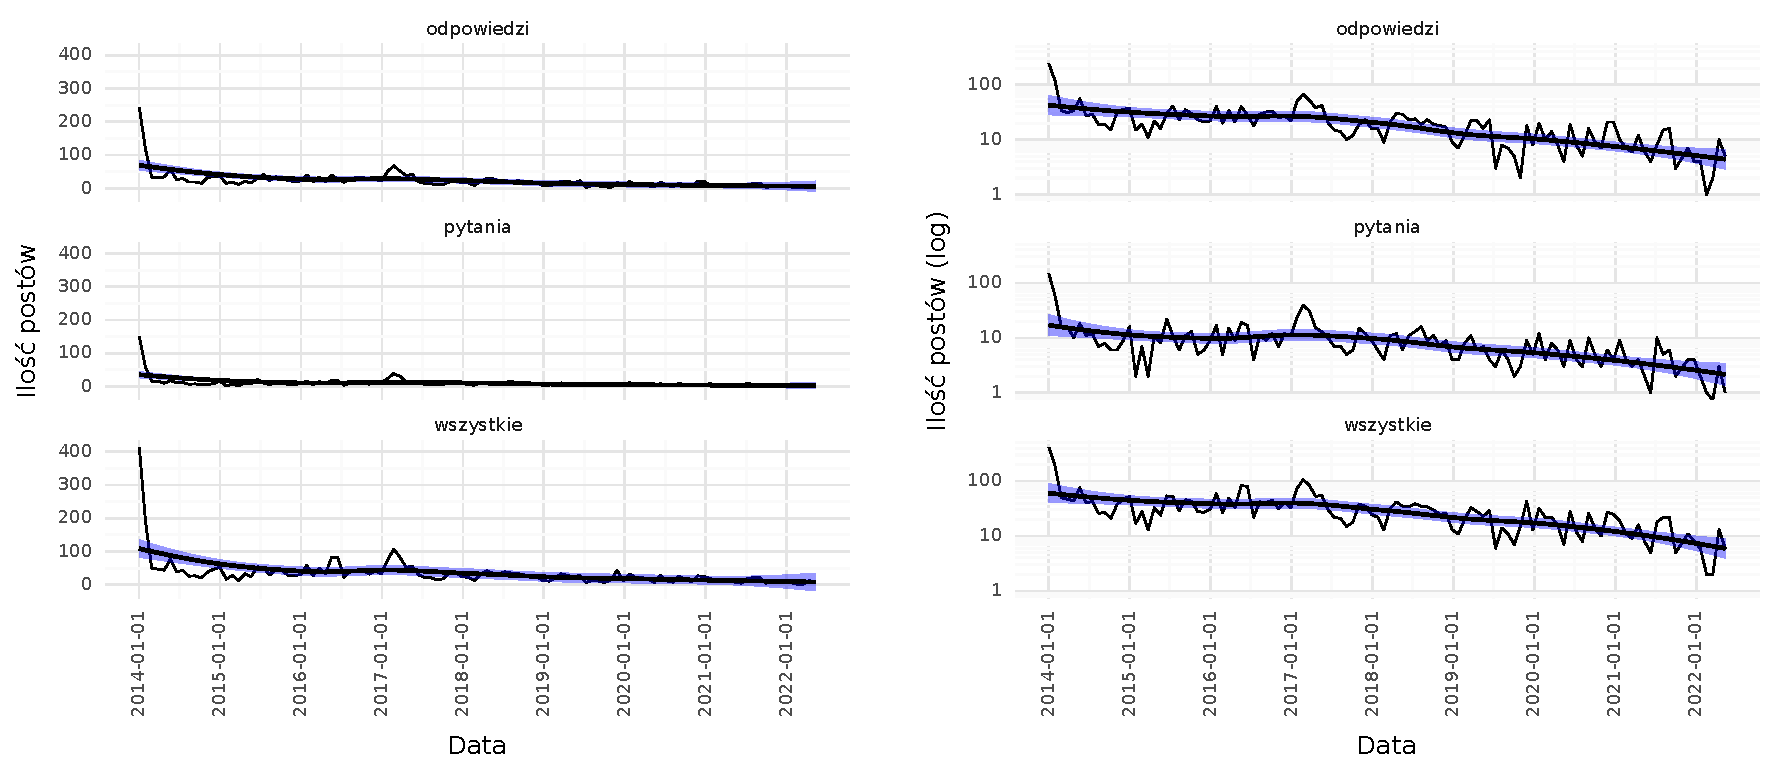
\includegraphics{./02_analytics_files/figure-pdf/fig-ryc2-output-1.pdf}

}

\caption{\label{fig-ryc2}Liczba postow w czasie z podzialem na pytania i
odpowiedzi. Lewy panel wskazuje surowe wartości liczby postów, prawy
wartości logarytmiczne o podstawie 10.}

\end{figure}

Stosunek ilości odpowiedzi do zadawanych pytań rośnie w czasie, lecz ma
na to wpływ zmniejszająca się ilość zadawanych pytań (maleje próba
badana) co zostało przedstawione na Rysunek~\ref{fig-ryc3}. Patrząc na
wartości średnie tylko co drugie pytanie uzyskiwało odpowiedź (ratio
0.48 +/- 0.22). Ogólne statystyki stosunku pytań do dopowiedzi w czasie
zostały przedstawione w Tabela~\ref{tbl-ratios}.

\begin{figure}

{\centering 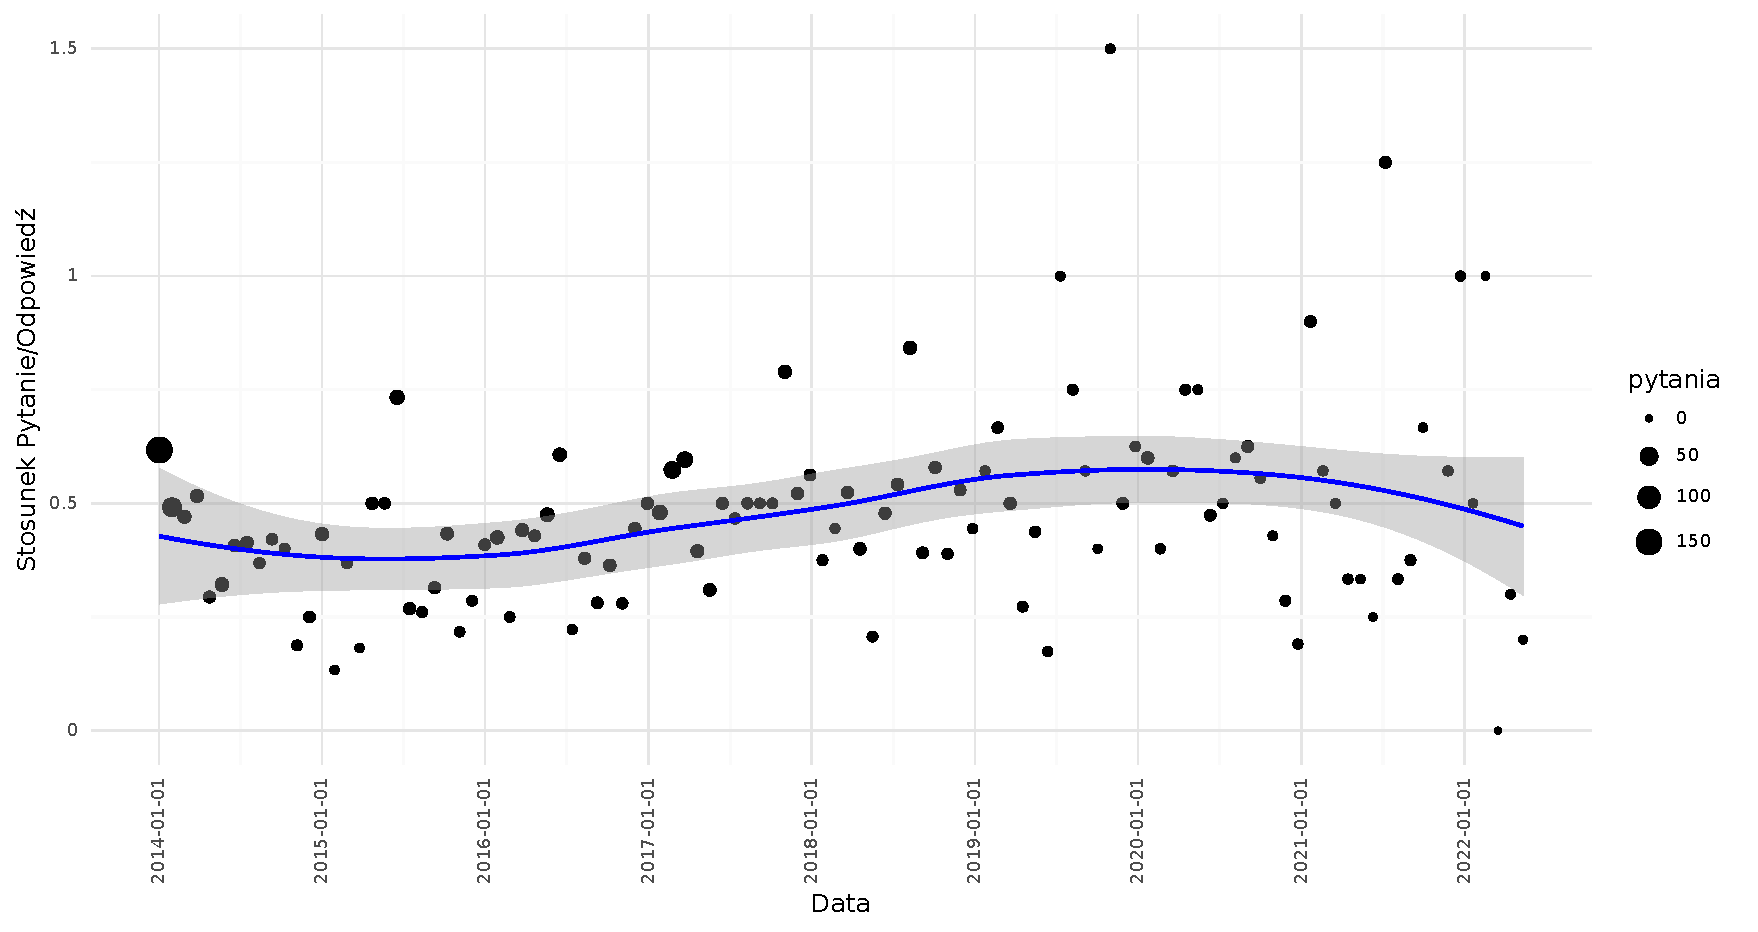
\includegraphics{./02_analytics_files/figure-pdf/fig-ryc3-output-1.pdf}

}

\caption{\label{fig-ryc3}Stosunek ilości odpowiedzi na zadane pytania w
czasie, uwzględniając ilość zadanych pytań}

\end{figure}

\hypertarget{tbl-ratios}{}
\begin{table}
\caption{\label{tbl-ratios}Statystyki stosunku ilości odpowiedzi na pytania. Bez uwzględnienia czy
było ono zaakceptowane czy też nie. }\tabularnewline

\centering
\begin{tabular}{lrrrrr}
\toprule
{} &   średnia &  odchylenie standardowe &  min &  max &   mediana \\
\midrule
0 &  0.476316 &                0.219824 &  0.0 &  1.5 &  0.444444 \\
\bottomrule
\end{tabular}
\end{table}

\hypertarget{dynamika-oraz-statystyki-udzielanych-odpowiedzi}{%
\section{Dynamika oraz statystyki udzielanych
odpowiedzi}\label{dynamika-oraz-statystyki-udzielanych-odpowiedzi}}

Twórcy pytań na forum mają możliwość wybrania odpowiedzi, która jest
najtrafniejsza i zawiera poprawną odpowiedź. Te odpowiedzi nazywane są
zaakceptowanymi odpowiedziami. Zbadano jak często najwyżej oceniona
odpowiedź nie była zaakceptowaną odpowiedzią.

Okazało się, że w przypadku pytań, które posiadały jakąkolwiek odpowiedź
około 12.7\% (646) przypadków najlepiej ocenianych odpowiedzi nie było
tą, która została zaakceptowana przez autora.

Następnie porównano oceny odpowiedzi zaakceptowanych z pozostałymi
odpowiedziami a statystyki przedstawiono w Tabela~\ref{tbl-a_stats} oraz
Rysunek~\ref{fig-ryc9}.

Pośród odpowiedzi na zadawane pytania wyróżniono 3 kategorie:

\begin{enumerate}
\def\labelenumi{\arabic{enumi}.}
\tightlist
\item
  odpowiedź zaakceptowana (\texttt{is\_accepted=True})
\item
  odpowiedź niezaakceptowana (\texttt{is\_accepted=False})
\item
  odpowiedź niezaakceptowana ale równocześnie brak jest zaakceptowanej
  odpowiedzi na to pytanie (\texttt{is\_accepted=None})
\end{enumerate}

Z analizy wynika, iż zaakceptowane odpowiedzi mają średnio wyższe oceny
użytkowników (6,39) niż pozostałe oceny (2.75 -
\texttt{is\_accepted=None}; 2.58 - \texttt{is\_accepted=False}), co było
oczekiwanym wynikiem.

\hypertarget{tbl-a_stats}{}
\begin{table}
\caption{\label{tbl-a_stats}Statystyki ocen odpowiedzi zaakceptowanych w stosunku do pozostałych }\tabularnewline

\centering
\begin{tabular}{llrrrrr}
\toprule
{} & is\_accepted &  avg\_score &  std\_score &  min\_score &  max\_score &  count(a\_id) \\
\midrule
0 &        None &   2.755169 &   3.181837 &         -5 &         30 &          919 \\
1 &        True &   6.395044 &   5.915949 &          0 &         46 &          686 \\
2 &       False &   2.584169 &   2.735329 &         -4 &         26 &          897 \\
\bottomrule
\end{tabular}
\end{table}

\begin{figure}

{\centering 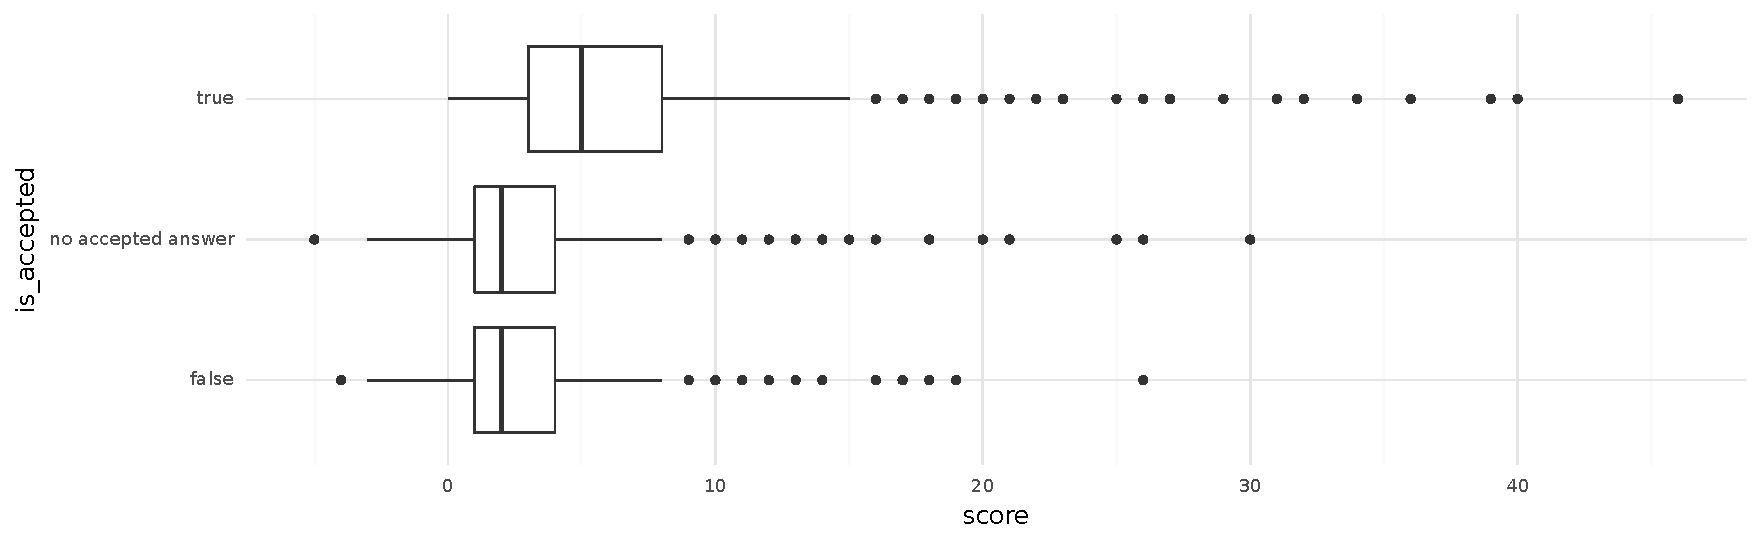
\includegraphics{./02_analytics_files/figure-pdf/fig-ryc9-output-1.pdf}

}

\caption{\label{fig-ryc9}Rozkład ocen pytań zaakceptowanych w porównaniu
do pozostałych}

\end{figure}

\begin{figure}

{\centering 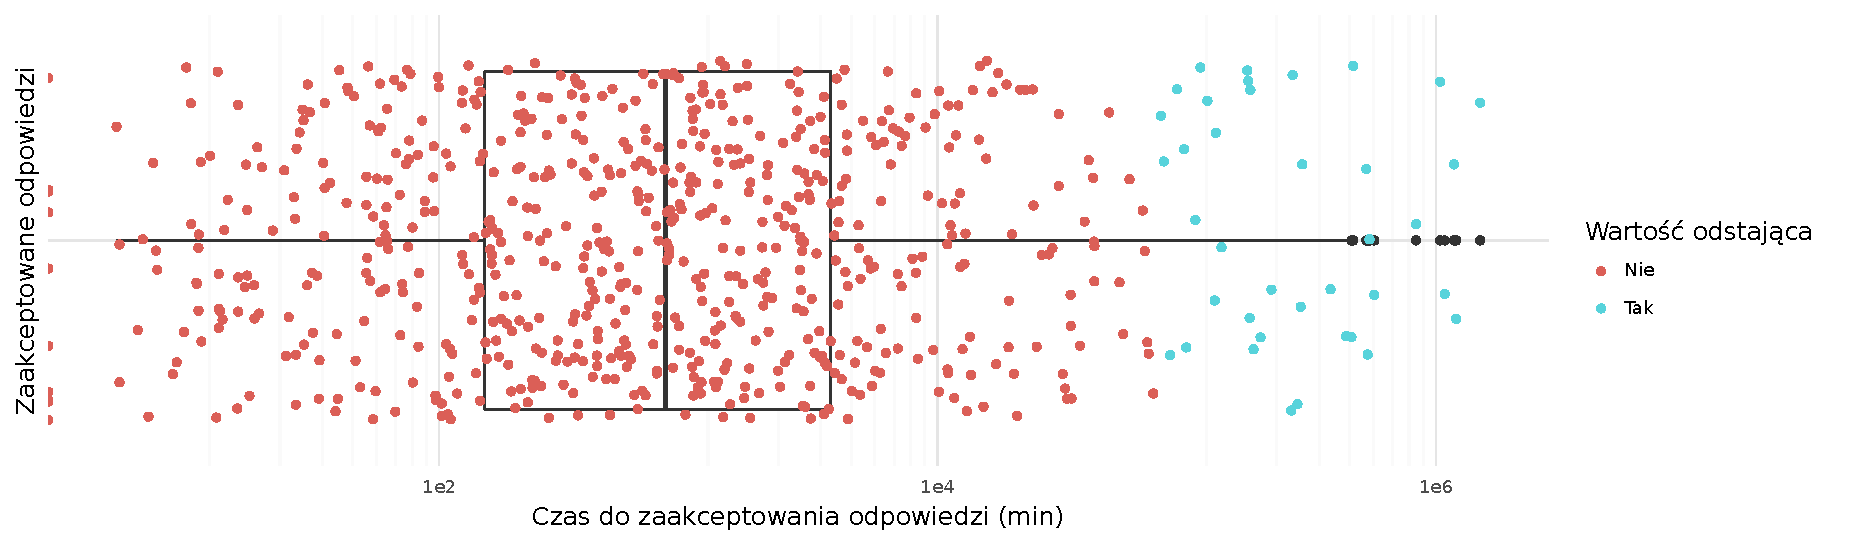
\includegraphics{./02_analytics_files/figure-pdf/fig-ryc10-output-1.pdf}

}

\caption{\label{fig-ryc10}Rozkład czasu od pojawienia się pytania do
zaakceptowanej odpowiedzi}

\end{figure}

\hypertarget{tbl-time_stats}{}
\begin{table}
\caption{\label{tbl-time_stats}Statystyki ocen odpowiedzi zaakceptowanych w stosunku do pozostałych }\tabularnewline

\centering
\begin{tabular}{lrrl}
\toprule
{} &  avg(time\_to\_accept\_min) &  stddev\_samp(time\_to\_accept\_min) &                 quantiles \\
\midrule
0 &             25244.943571 &                     123338.63251 &  [141.53, 753.25, 3605.8] \\
\bottomrule
\end{tabular}
\end{table}

\hypertarget{tbl-time_stats_no_outliers}{}
\begin{table}
\caption{\label{tbl-time_stats_no_outliers}Statystyki ocen odpowiedzi zaakceptowanych w stosunku do pozostałych po
odrzuceniu wartości odstających \textgreater{} 100000 }\tabularnewline

\centering
\begin{tabular}{lrrl}
\toprule
{} &  avg(time\_to\_accept\_min) &  stddev\_samp(time\_to\_accept\_min) &                  quantiles \\
\midrule
0 &              4769.308792 &                     12694.627624 &  [127.72, 644.93, 2922.82] \\
\bottomrule
\end{tabular}
\end{table}

Następnie zbadano jak szybko od pojawienia się pytania, pojawia się
zaakceptowana odpowiedź. Dla wszystkich pytań na tym forum jest to
średnio 25244 minuty, ale wartość środkowa (753) sugeruje, że średnia
może być zaburzona. W celu obliczenia średniej nie zaburzonej tak dużymi
wartościami odstającymi odrzucono wartości powyżej 100000 minut. Tym
razem uzyskano wartość 4769 minut (\textasciitilde3 dni), przy wartości
środkowej 644 (\textasciitilde10 godzin).

Rozkłady wartości przedstawiono na Rysunek~\ref{fig-ryc10} oraz w
Tabela~\ref{tbl-time_stats} dla całego zbioru danych oraz
Tabela~\ref{tbl-time_stats_no_outliers} po odrzuceniu wartości
odstających.

\hypertarget{retencja-uux17cytkownikuxf3w}{%
\section{Retencja użytkowników}\label{retencja-uux17cytkownikuxf3w}}

W całej historii forum zarejestrowanych zostało 8948 użytkowników, z
czego jedno konto jest kontem bota. Miarą retencji użytkownika na forum
określono czas od utworzenia konta to ostaniej zamieszczonej wiadomości.
Wśród 50 najdłużej aktywnych kont zidentyfikowano konto z wynikiem aż
3052 dni a konto z ostatnim indeksem w tej grupie miało wynik 2128 dni.
Jednakże patrząc na całą populację, wartość środkowa wyniosła 11, a 50\%
wartości mieści się pomiędzy 0 a 594 dniami. Użytkownicy z wartością 0,
są to najprawdopodobniej użytkowicy, którzy zadali jedyne pytanie na
forum w dniu założenia konta (410 użytkowników). Czas na forum najdłużej
aktywnych użytkowników został zwizualizowany na Rysunek~\ref{fig-ryc4}.
Dodatkowo okazało się, że 7691 (86\%) kont było biernymi użytkownikami
forum i nidgy nie dodało żadnego posta.

\begin{figure}

{\centering 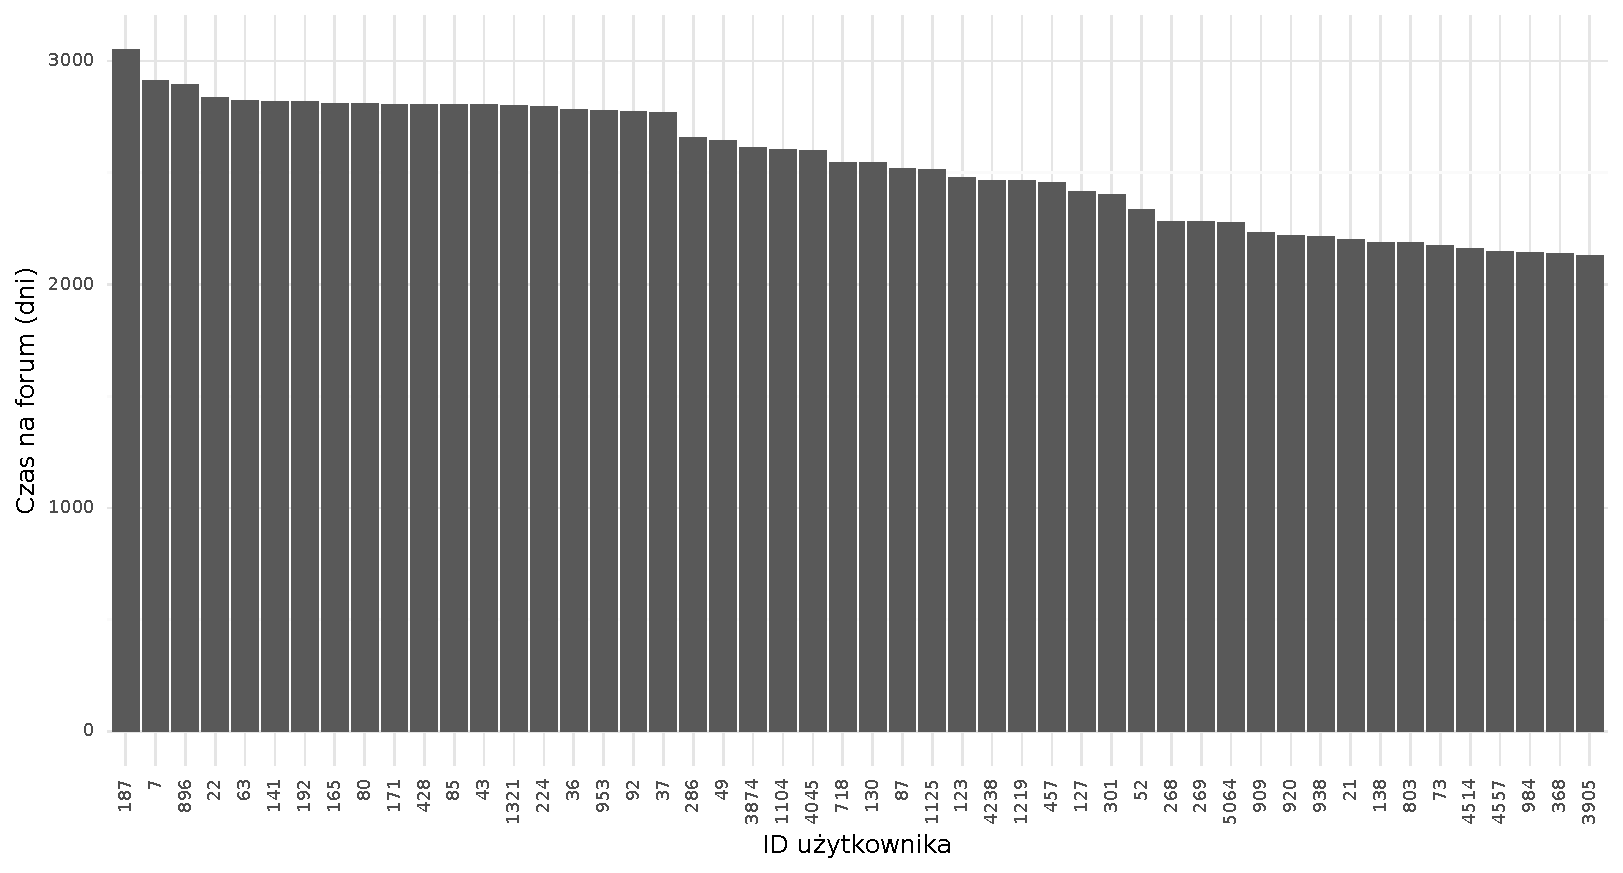
\includegraphics{./02_analytics_files/figure-pdf/fig-ryc4-output-1.pdf}

}

\caption{\label{fig-ryc4}Czas na forum 50 najdłużej aktywnych kont}

\end{figure}

\hypertarget{sec-qstats}{%
\section{Statystyki najwyżej oraz najniżej ocenianych
pytań}\label{sec-qstats}}

Zbadano statystyki zadawanych pytań. Użytkownicy forum mogą oceniać
pojawiające się tam pytania czego miarą jest wartość \texttt{score}.
Sprawdzono, czy długość zadanego pytania ma wpływ na jego ocenę.

Średnia długość pytania wyniosła 415 znaków (+/- 330) a wartość środkowa
331 znaków. Najdłuższe pytanie posiadało 3133 znaki a najkrótsze jedynie
30. Statystyki przedstawiono w Tabela~\ref{tbl-q_stats}.

\hypertarget{tbl-q_stats}{}
\begin{table}
\caption{\label{tbl-q_stats}Statystyki długości postów }\tabularnewline

\centering
\begin{tabular}{lrrrrr}
\toprule
{} &     średnia &  odchylenie standardowe &   max &  min &  mediana \\
\midrule
0 &  415.863676 &              330.836043 &  3133 &   30 &      331 \\
\bottomrule
\end{tabular}
\end{table}

Średnio pytanie było oceniane na wartość 6.28 (+/-5.88) a wartość
środkowa wyniosła 5. Najlepiej oceniane pytanie miało ocenę 67 a
najgorzej -7. Statystyki zestawiono w Tabela~\ref{tbl-score_stats}.

\hypertarget{tbl-score_stats}{}
\begin{table}
\caption{\label{tbl-score_stats}Statystyki ocen użytkowników }\tabularnewline

\centering
\begin{tabular}{lrrrrr}
\toprule
{} &   średnia &  odchylenie standardowe &  max &  min &  mediana \\
\midrule
0 &  6.278804 &                5.876114 &   68 &   -7 &        5 \\
\bottomrule
\end{tabular}
\end{table}

Zależność pomiędzy wartością \texttt{score} a długością wiadomości
przedstawiono na Rysunek~\ref{fig-ryc5}. Ze względu na obecność dużej
ilości wartości odstających obie wartości przedstawiono również w skali
logarymicznej.

Nie wykryto korelacji pomiędzy tymi dwoma zmiennymi. Współczynnik
korelacji wyniósł -0.048 oraz -0.018 dla wartości zlogarytmowanych.

Postanowiono dodatkowo zbadać dwie podgrupy danych dla pytań najlepiej
oraz najgorzej ocenianych. Wyodrębniono po 100 pytań z każdej z grup.
Wyniki dla tych grup przestwationo na Rysunek~\ref{fig-ryc5} (dolny
panel) oraz w Tabela~\ref{tbl-q_stats_types} i
Tabela~\ref{tbl-score_stats_types}.

W podgrupie najlepiej ocenianych pytań średnia ocena wyniosła 20.6 +/-
8.5 a w podgrupie najgorzej ocenianych 0.4 +/- 1.2. Rozdzielność tych
statystyk dla tych grup była oczekiwanym wynikiem.

Statystyki długości pytań nie odbiegają od siebie w znaczący sposób
(średnie 349 +/- 275 najlepiej oceniane oraz 389 +/- 424 najgorzej
oceniane) sugerując iż to długość pytania nie ma znaczącego wpływu na
jego ocenę.

\begin{figure}

{\centering 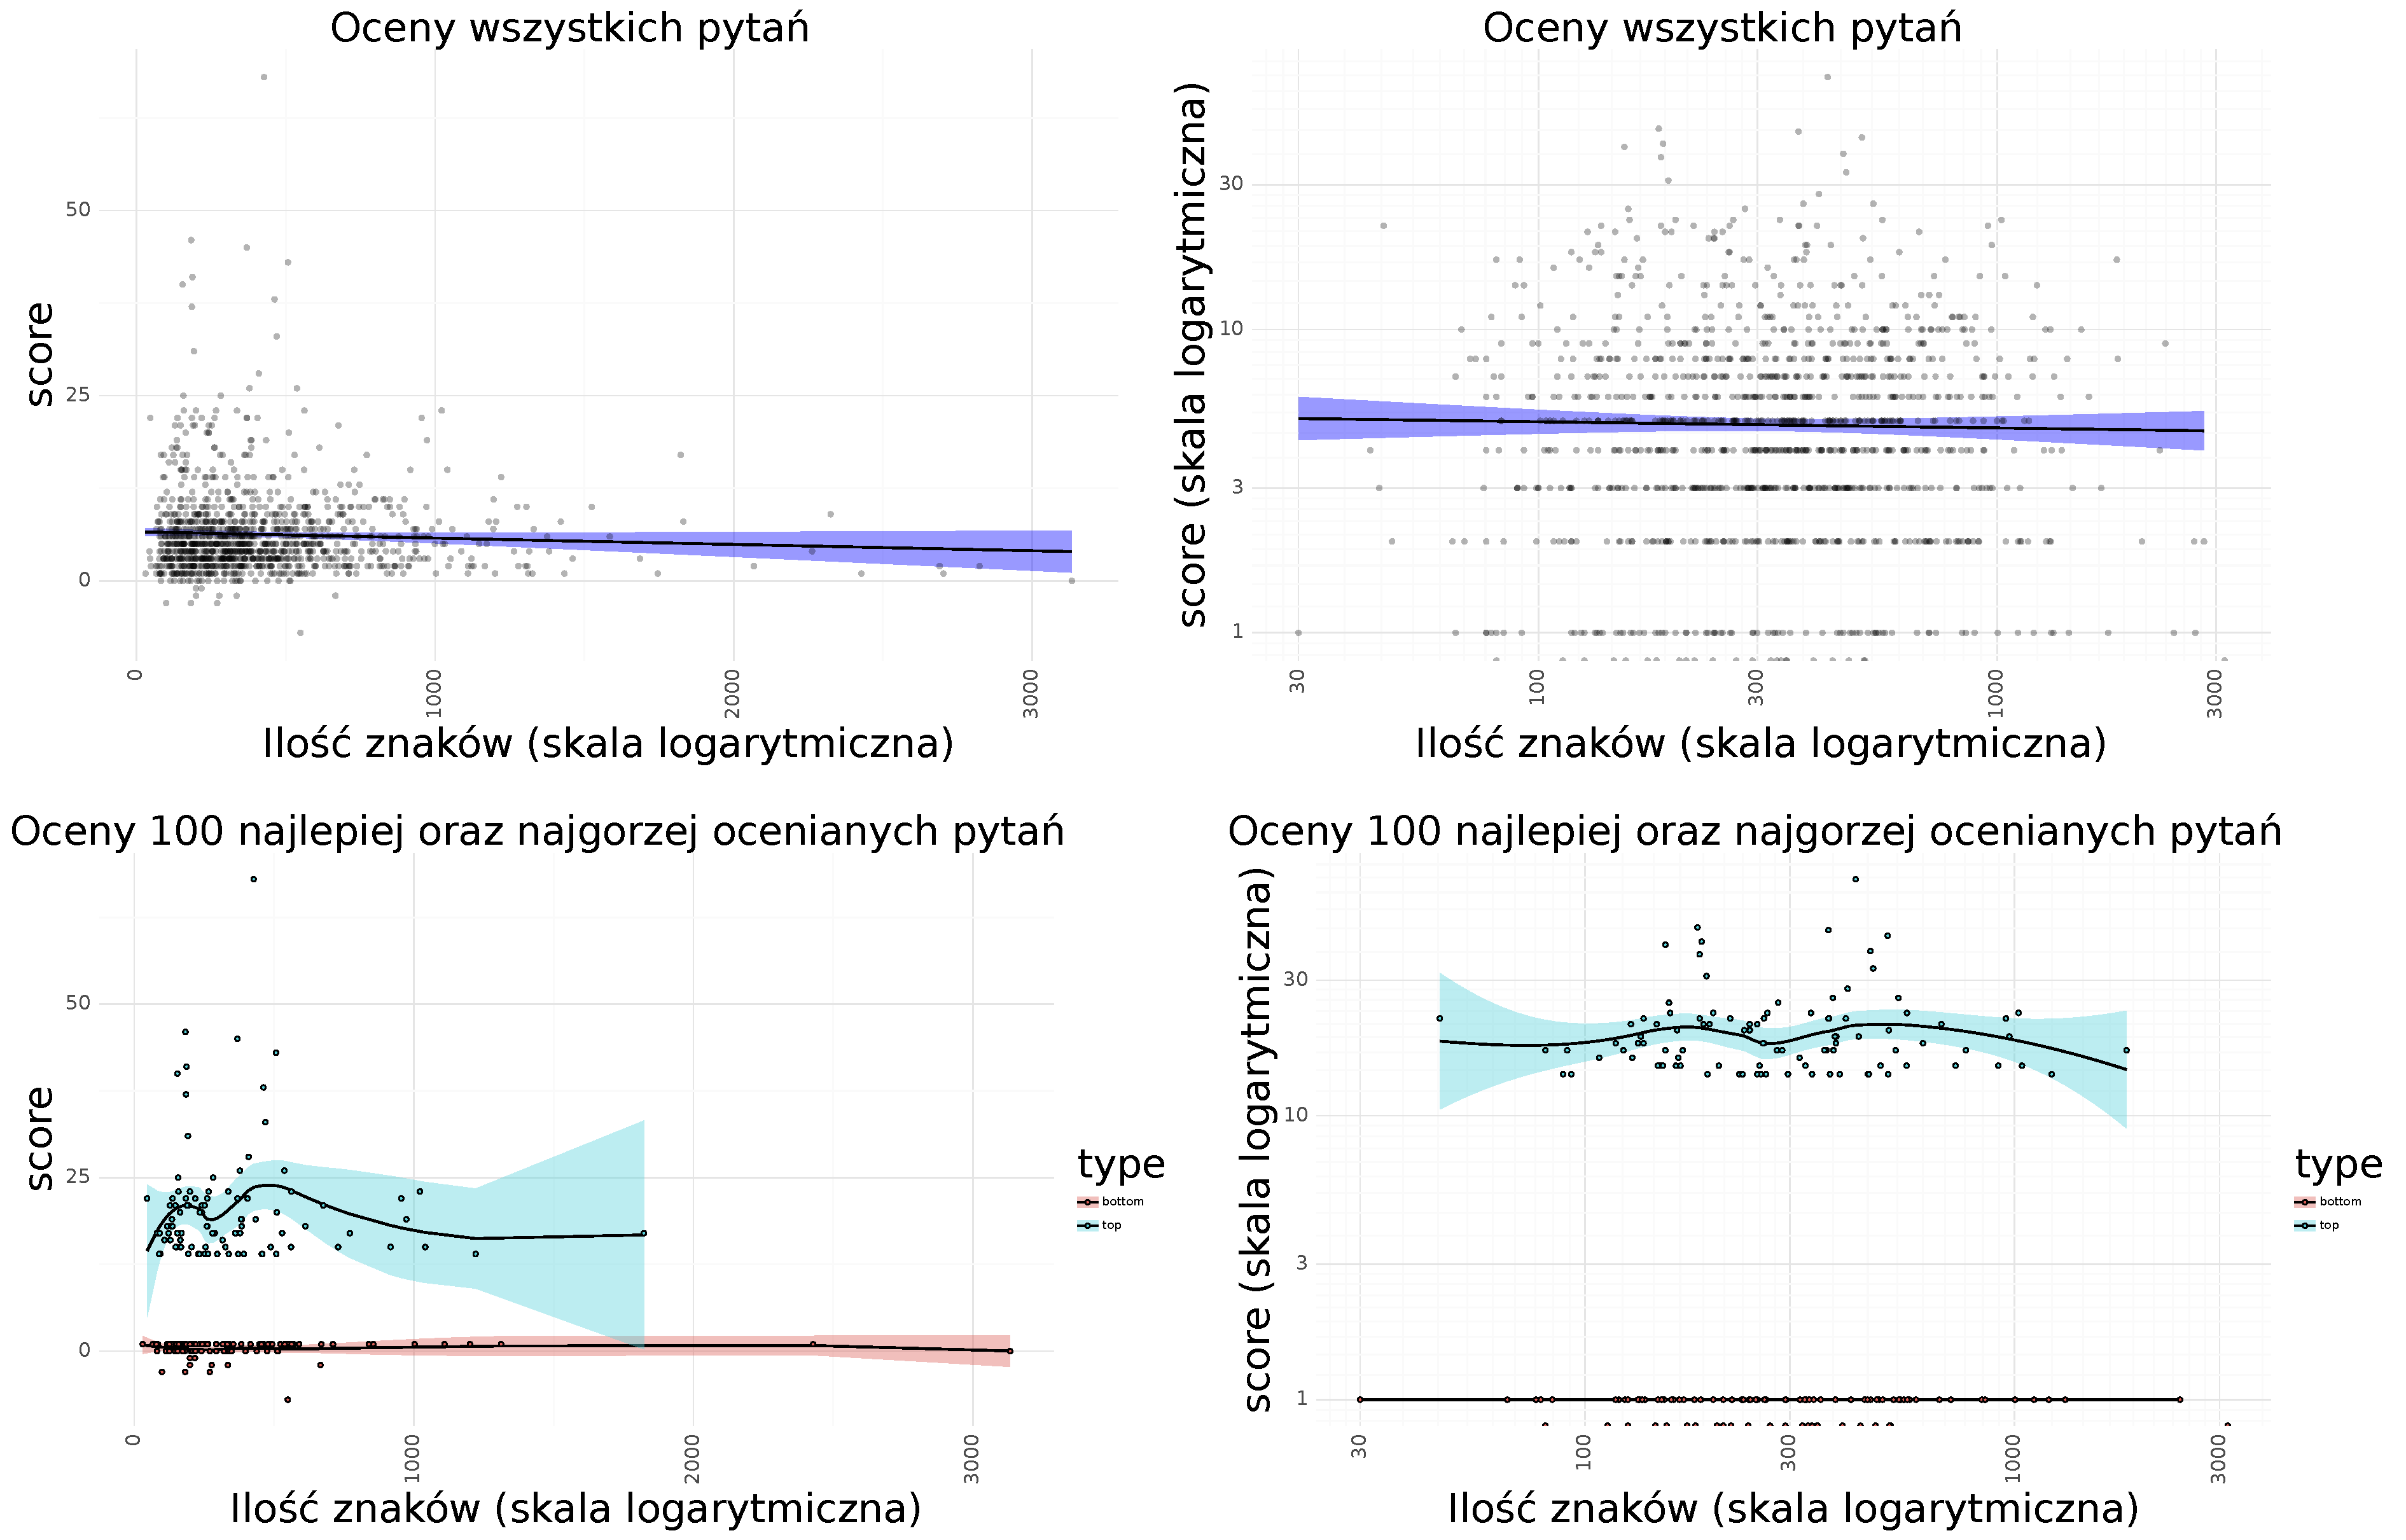
\includegraphics{./02_analytics_files/figure-pdf/fig-ryc5-output-1.pdf}

}

\caption{\label{fig-ryc5}Oceny pytań na forum w zależności od długości
zadanego pytania}

\end{figure}

\hypertarget{tbl-q_stats_types}{}
\begin{table}
\caption{\label{tbl-q_stats_types}Statystyki długości postów z podziałem na podgrupy najlepszych i
najgorszych pytań }\tabularnewline

\centering
\begin{tabular}{llrrrrr}
\toprule
{} &    type &  średnia &  odchylenie standardowe &   max &  min &  mediana \\
\midrule
0 &     top &   349.08 &              275.088587 &  1823 &   46 &      261 \\
1 &  bottom &   389.26 &              424.654836 &  3133 &   30 &      270 \\
\bottomrule
\end{tabular}
\end{table}

\hypertarget{tbl-score_stats_types}{}
\begin{table}
\caption{\label{tbl-score_stats_types}Statystyki ocen użytkowników z podziałem na podgrupy najlepszych i
najgorszych pytań }\tabularnewline

\centering
\begin{tabular}{llrrrrr}
\toprule
{} &    type &  średnia &  odchylenie standardowe &  max &  min &  mediana \\
\midrule
0 &     top &     20.6 &                8.551685 &   68 &   14 &       18 \\
1 &  bottom &      0.4 &                1.206045 &    1 &   -7 &        1 \\
\bottomrule
\end{tabular}
\end{table}

Zauważono również że najlepiej oceniane pytania są również częściej
oglądane i mają więcej odpowiedzi niż pytania najgorzej oceniane
(Rysunek~\ref{fig-ryc6}). Najlepiej oceniane pytania mają średnio 17
odpowiedzi podczas gdy najgorzej jedynie 4
(Tabela~\ref{tbl-answers_stats_types}) oraz odpowiednio średnio 26289 i
475 wyświetleń (Tabela~\ref{tbl-views_stats_types})

\begin{figure}

{\centering 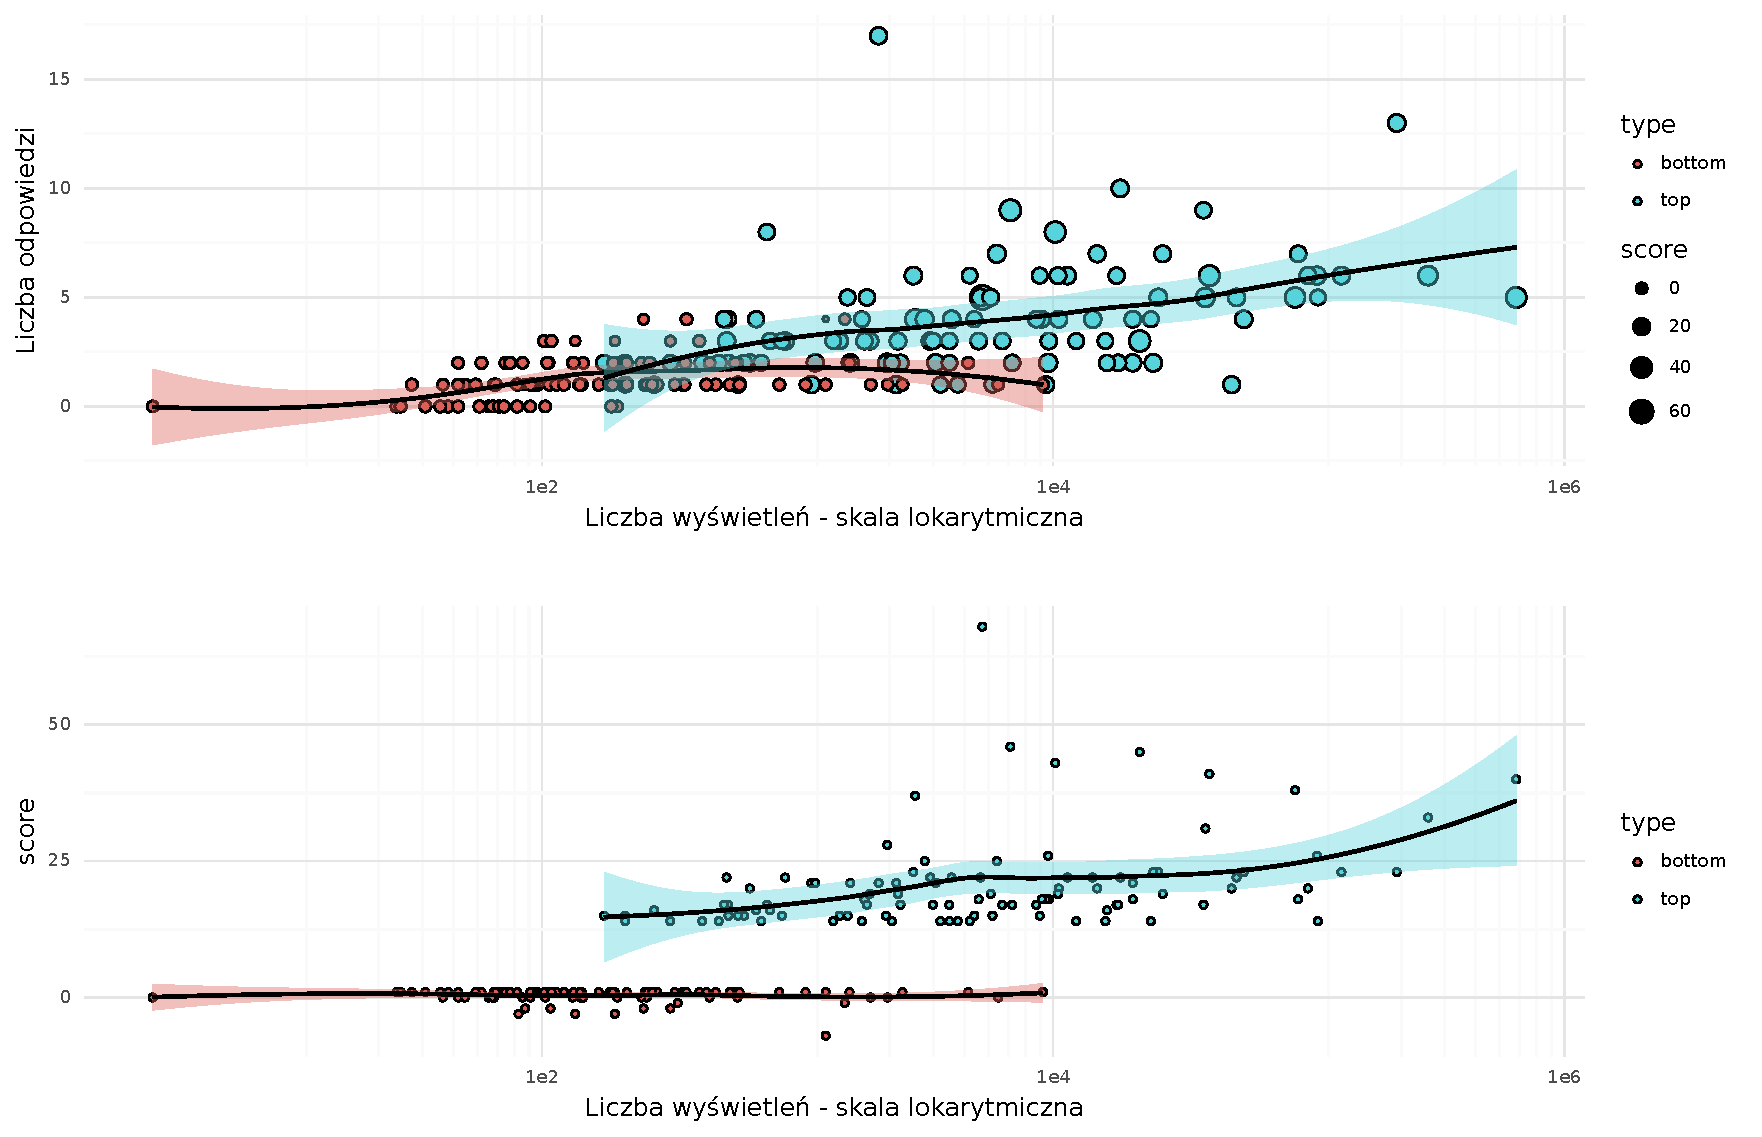
\includegraphics{./02_analytics_files/figure-pdf/fig-ryc6-output-1.pdf}

}

\caption{\label{fig-ryc6}Oceny pytań na forum w zależności od ilości
wyświetleń i odpowiedzi}

\end{figure}

\hypertarget{tbl-answers_stats_types}{}
\begin{table}
\caption{\label{tbl-answers_stats_types}Statystyki ilości odpowiedzi na pytania z podziałem na podgrupy
najlepszych i najgorszych pytań }\tabularnewline

\centering
\begin{tabular}{llrrrrr}
\toprule
{} &    type &  max(answer\_count) &  min(answer\_count) &  mean &   std\_dev &  median \\
\midrule
0 &     top &                 17 &                  1 &  3.96 &  2.581676 &       3 \\
1 &  bottom &                  4 &                  0 &  1.28 &  0.964836 &       1 \\
\bottomrule
\end{tabular}
\end{table}

\hypertarget{tbl-views_stats_types}{}
\begin{table}
\caption{\label{tbl-views_stats_types}Statystyki ilości wyświetleń pytań z podziałem na podgrupy najlepszych i
najgorszych pytań }\tabularnewline

\centering
\begin{tabular}{llrrrrr}
\toprule
{} &    type &  max(view\_count) &  min(view\_count) &      mean &       std\_dev &  median \\
\midrule
0 &     top &           648941 &              175 &  26047.65 &  76276.200191 &    4715 \\
1 &  bottom &             9124 &                3 &    495.56 &   1220.756292 &     141 \\
\bottomrule
\end{tabular}
\end{table}

\hypertarget{analiza-znacznikuxf3w-taguxf3w}{%
\section{Analiza znaczników
(tagów)}\label{analiza-znacznikuxf3w-taguxf3w}}

W celu identyfikacji tematów zapytań na forum przeanalizowano słowa
kluczowe, którymi oznaczano pytania. Wyniki przedstawiono w postaci
wykresu typu ``Chmura słów'' Rysunek~\ref{fig-ryc7}. Okazuje się, że
użytkownicy najczęściej pytali o \texttt{wina} (134, ang. \emph{wine}),
\texttt{smak} (120, ang. \emph{taste}), \texttt{historię} (85, ang.
\emph{history}) i o \texttt{rekomendacje} (76, ang.
\emph{recommandation}).

Tę samą analizę wykonano na grupie 100 najlepiej i najgorzej ocenianych
pytań badanych w Sekcja~\ref{sec-qstats}. W pierwszej grupie najczęściej
używano znaczników \texttt{smak} (17) oraz \texttt{warzenie} (14, ang.
\emph{brewing}), w drugiej natomiast najczęściej pytano o \texttt{wina}
(20), \texttt{rekomendacje} (15) i \texttt{zdrowie} (12, ang.
\emph{health}).

\begin{figure}

{\centering 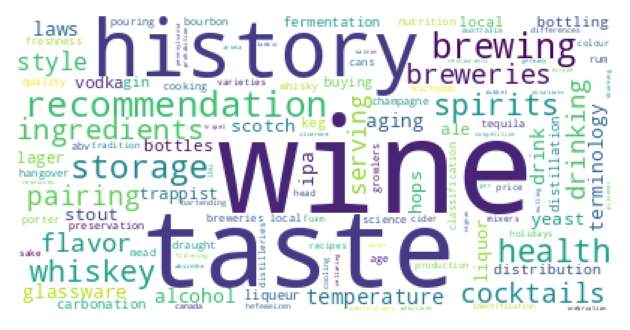
\includegraphics{./02_analytics_files/figure-pdf/fig-ryc7-output-1.pdf}

}

\caption{\label{fig-ryc7}Chmura słów przedstawiająca najczęściej używane
znaczniki na forum}

\end{figure}

Następnie sprawdzono, które ze znaczników nie tylko były najczęściej
używane, lecz które generowały najwięcej wyświetleń. W tym celu
zsumowano liczbę wyświetleń wszystkich zapytań na forum, w którym
pojawił się dany znacznik (Tabela~\ref{tbl-tags_views}). Znaczniki
\texttt{taste} oraz \texttt{health} generują najwięcej wyświetleń na tym
forum w ilości 1349051 oraz 1316064, na dalszych miejscach znajdują się
znaczniki \texttt{preservation} (686106), \texttt{storage} (558949) oraz
\texttt{whiskey}(470841).

\hypertarget{tbl-tags_views}{}
\begin{table}
\caption{\label{tbl-tags_views}Sumaryczne ilości wyświetleń wiadomości zawierających dany znacznik.
Przedstawiono 10 najpopularniejszych znaczników. }\tabularnewline

\centering
\begin{tabular}{llr}
\toprule
{} &           tag &  sum\_views \\
\midrule
0 &         taste &    1330670 \\
1 &        health &    1286001 \\
2 &  preservation &     682216 \\
3 &       storage &     542860 \\
4 &       whiskey &     464756 \\
5 &       bourbon &     330268 \\
6 &       brewing &     307892 \\
7 &           ipa &     291935 \\
8 &       spirits &     255328 \\
9 &      drinking &     225924 \\
\bottomrule
\end{tabular}
\end{table}

Zbadano również czy wykorzystanie najczęściej używanych znaczników
zmieniało się w czasie istnienia forum. Z danych zaprezentowanych na
Rysunek~\ref{fig-ryc8} można zaobserwować że niektóre znaczniki takie
jak \texttt{spirits}, \texttt{bourbon} czy \texttt{whiskey} zaczęły być
używane dopiero około roku 2016 - około 2 lata po pierwszej wiadomości
na forum. W danych zauważono również, że częstość używania znaczników
jest skokowa. Może to być związane z ogólną małą ilością postów
zamieszczanych na forum. Wyjątek stanowią najpopularniejsze znaczniki,
takie jak \texttt{taste} czy \texttt{health}, których częstość
występowania jest bardziej regularna.

\begin{figure}

{\centering 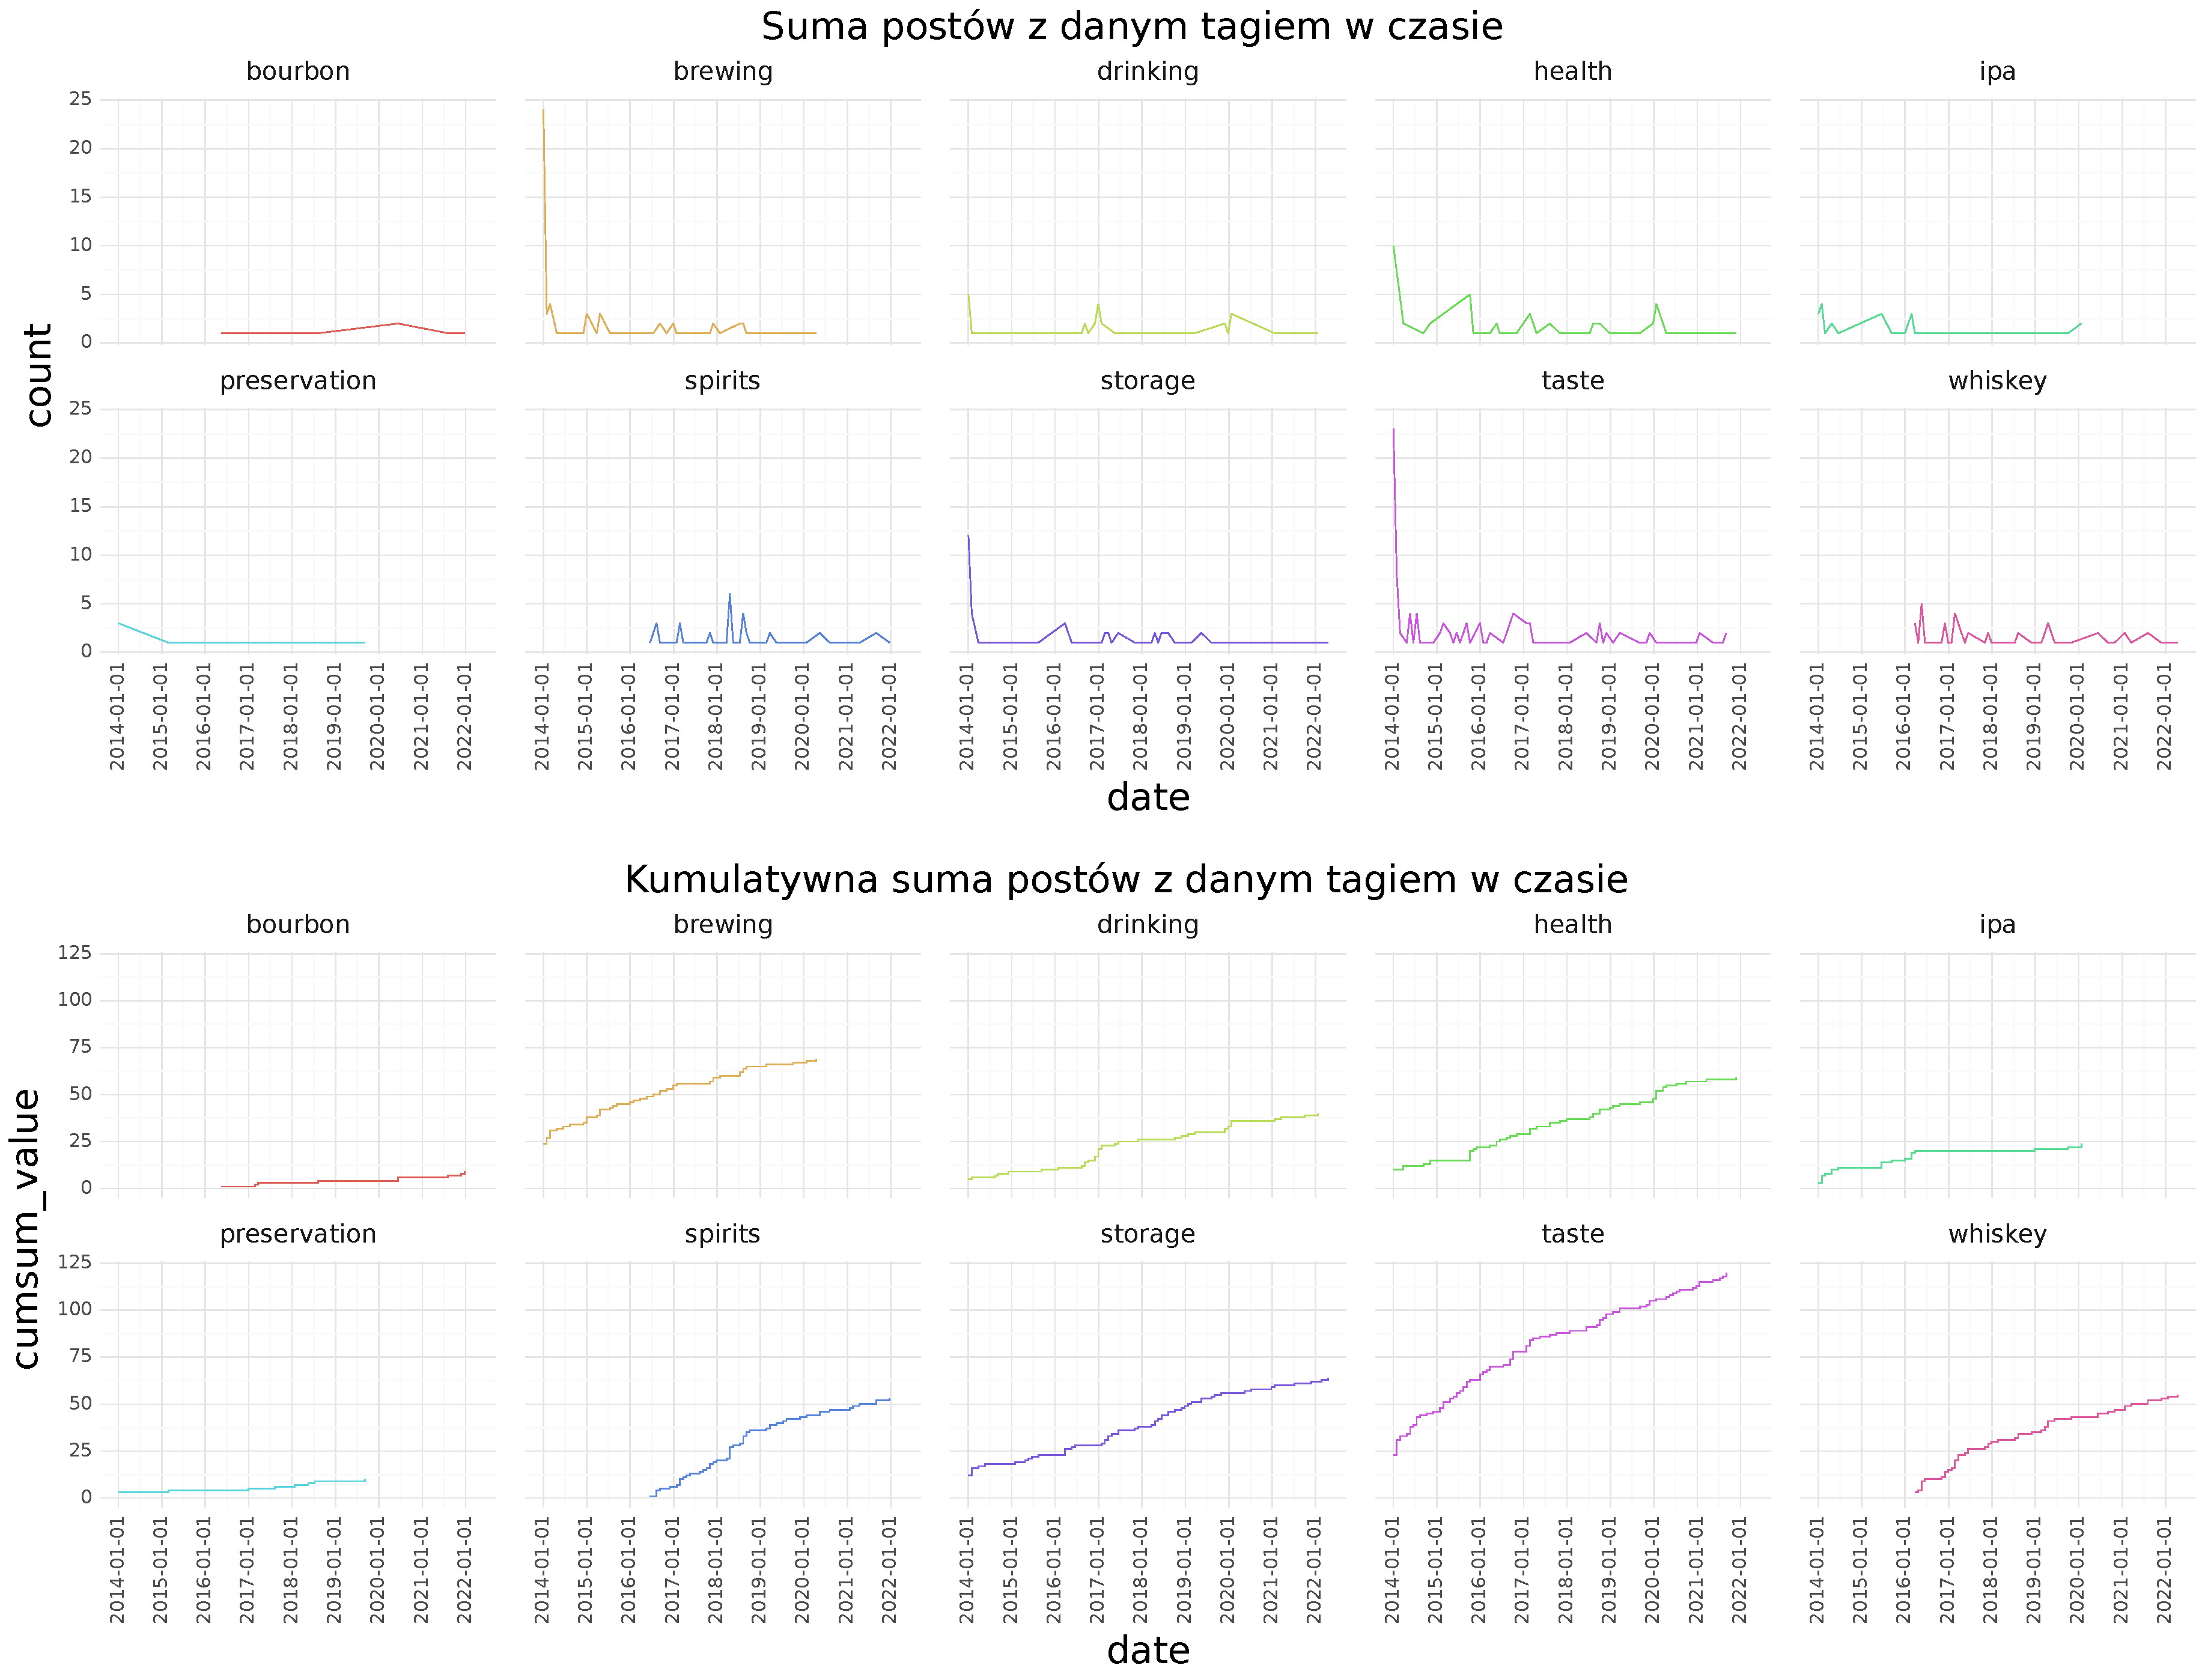
\includegraphics{./02_analytics_files/figure-pdf/fig-ryc8-output-1.pdf}

}

\caption{\label{fig-ryc8}Liczba postów w czasie dla każdego z
najczęściej wyświetlanych znaczników. Wartości zagregowane na poziomie
miesięcy. Górny panel przedstawia wartości miesięczne, dolny natomiast
miesięczną sumę kumulatywną.}

\end{figure}

\hypertarget{analiza-tytuux142uxf3w-postuxf3w}{%
\section{Analiza tytułów
postów}\label{analiza-tytuux142uxf3w-postuxf3w}}

Dodatkową metodą, oprócz analizy znaczkików, którą można wykorzystać w
celu zbadania tematów poruszanych na forum może być analiza najczęściej
pojawiających się słów. Można do tego wykorzystać treść tytułów
wiadomości jak i ich główną treść. W niniejszej pracy skupiono się na
analizie treści tytułów wiadomości, jako że bardzo często zawierają one
dużo słów kluczowych.

Tytuły wiadomości są nieustrukturyzowanymi ciągami znaków, z tego powodu
do ich analizy wykorzystano powszechnie używane narzędzia stosowane przy
analizach NLP (ang. \emph{\textbf{N}atural \textbf{L}anguage
\textbf{P}rocessing}). Proces zastosowanej tutaj analizy tekstu składał
się z 4 kroków:

\begin{enumerate}
\def\labelenumi{\arabic{enumi}.}
\tightlist
\item
  Wyodrębnienia tokenów
\item
  Usunięcia tokenów o długości znaku 1
\item
  Usunięcia tokenów nie niosących informacji o treści (ang. \emph{stop
  words})
\item
  Ujednolicenia różych form danego wyrazu poprzez zabieg stemming'u
  (ang. \emph{stemming}), mającego na celu ucinanie końcówek wyrazów
  (tokenów) i pozostawieniu jedynie jego wartości bazowej.
\end{enumerate}

Przykładowa tabela wizualizująca tokeny surowe w porównaniu do tokenów
po odfiltrowaniu słów typu \texttt{stop\ words} oraz tokenów krótszych
niż 1 zaprezentowano na Tabela~\ref{tbl-tokens}

\hypertarget{tbl-tokens}{}
\begin{table}
\caption{\label{tbl-tokens}Przykładowe rekordy danych wizualizujące proces przetwarzania tekstu.
Kolejność chronologiczna kolumn title --\textgreater{} words\_token
--\textgreater{} words\_no\_stop --\textgreater{} words\_stem }\tabularnewline

\centering
\begin{tabular}{ll}
\toprule
{} &                                                                      0 \\
\midrule
title         &           What is a citra hop, and how does it differ from other hops? \\
words\_token   &  [what, is, citra, hop, and, how, does, it, differ, from, other, hops] \\
words\_no\_stop &                                             [citra, hop, differ, hops] \\
words\_stem    &                                              [citra, hop, differ, hop] \\
\bottomrule
\end{tabular}
\end{table}

Dzięki zabiegowi stemmingu otrzymywany jest bardziej jednorodny zestaw
danych. Liczba unikalnych tokenów została zredukowana z 2055 do 1680.

Następnie zliczono, które tokeny pojawiają się w największej ilości
tytułów i zaprezentowano w Tabela~\ref{tbl-tokens_count}. Najczęściej
używanymi tokenami były tokeny \texttt{beer} (476), \texttt{wine} (152)
oraz \texttt{drink} (105). Wyniki pozostają w zgodzie z wnioskami
uzyskanymi poprzez analizę znaczników.

\hypertarget{tbl-tokens_count}{}
\begin{table}
\caption{\label{tbl-tokens_count}Zliczenia tokenów słów najczęściej pojawiających się w tytułach postów
(15 najliczniejszych) }\tabularnewline

\centering
\begin{tabular}{llr}
\toprule
{} &      words &  count \\
\midrule
0  &       beer &    476 \\
1  &       wine &    147 \\
2  &      drink &    104 \\
3  &    alcohol &     88 \\
4  &     differ &     72 \\
5  &      bottl &     68 \\
6  &        use &     50 \\
7  &       tast &     47 \\
8  &       brew &     43 \\
9  &       make &     41 \\
10 &       good &     33 \\
11 &   cocktail &     29 \\
12 &        age &     27 \\
13 &        ale &     26 \\
14 &  recommend &     26 \\
\bottomrule
\end{tabular}
\end{table}

\bookmarksetup{startatroot}

\hypertarget{bibliografia}{%
\chapter*{Bibliografia}\label{bibliografia}}
\addcontentsline{toc}{chapter}{Bibliografia}

\markboth{Bibliografia}{Bibliografia}

\hypertarget{refs}{}
\begin{CSLReferences}{0}{0}
\end{CSLReferences}

\bookmarksetup{startatroot}

\hypertarget{sec-appendix}{%
\chapter{Załączniki}\label{sec-appendix}}

\hypertarget{polecenia-budujux105ce-infrastrukturux119}{%
\section{Polecenia budujące
infrastrukturę}\label{polecenia-budujux105ce-infrastrukturux119}}

\hypertarget{sec-emr}{%
\subsection{EMR}\label{sec-emr}}

\small

\begin{Shaded}
\begin{Highlighting}[]
\ExtensionTok{aws}\NormalTok{ emr create{-}cluster }\AttributeTok{{-}{-}name}\OperatorTok{=}\StringTok{"MyEMRCluster"} \DataTypeTok{\textbackslash{}}
    \AttributeTok{{-}{-}release{-}label}\NormalTok{ emr{-}6.8.0 }\DataTypeTok{\textbackslash{}}
    \AttributeTok{{-}{-}applications}\NormalTok{ Name=JupyterHub Name=Hadoop Name=Spark }\DataTypeTok{\textbackslash{}}
    \AttributeTok{{-}{-}log{-}uri}\NormalTok{ s3://emr{-}logs{-}beer{-}and{-}wine/MyJupyterClusterLogs }\DataTypeTok{\textbackslash{}}
    \AttributeTok{{-}{-}use{-}default{-}roles} \DataTypeTok{\textbackslash{}}
    \AttributeTok{{-}{-}instance{-}groups}\NormalTok{ InstanceGroupType=MASTER,InstanceCount=1,InstanceType=m4.large InstanceGroupType=CORE,InstanceCount=2,InstanceType=m4.large }\DataTypeTok{\textbackslash{}}
    \AttributeTok{{-}{-}ebs{-}root{-}volume{-}size}\NormalTok{ 32 }\DataTypeTok{\textbackslash{}}
    \AttributeTok{{-}{-}configurations}\NormalTok{ file://emr{-}configurations.json }\DataTypeTok{\textbackslash{}}
    \AttributeTok{{-}{-}bootstrap{-}actions}\NormalTok{ Path=s3://misc{-}beer{-}and{-}wine/install\_python\_libraries.sh,Name=InstallJupyterLibs}
\end{Highlighting}
\end{Shaded}

\normalsize

Plik \texttt{install-my-jupyter-libraries.sh} dostępny jest pod
poniższym \href{}{adresem}

\hypertarget{s3}{%
\subsection{S3}\label{s3}}

Koszyki S3 zostały utworzone przy pomocy poniższego polecenia:

\begin{verbatim}
aws s3api create-bucket --acl private --bucket <nazwa koszka>
\end{verbatim}

\hypertarget{definicje-funkcji}{%
\section{Definicje funkcji}\label{definicje-funkcji}}

\hypertarget{sec-tags-remove}{%
\subsection{tags\_remove()}\label{sec-tags-remove}}

\begin{Shaded}
\begin{Highlighting}[]
\ImportTok{from}\NormalTok{ pyspark.sql.functions }\ImportTok{import}\NormalTok{ udf}
\ImportTok{from}\NormalTok{ bs4 }\ImportTok{import}\NormalTok{ BeautifulSoup}
\ImportTok{from}\NormalTok{ html }\ImportTok{import}\NormalTok{ unescape}

\KeywordTok{def}\NormalTok{ tags\_remove(s):}
    \ControlFlowTok{if}\NormalTok{ s }\KeywordTok{is} \KeywordTok{not} \VariableTok{None}\NormalTok{:}
\NormalTok{        soup }\OperatorTok{=}\NormalTok{ BeautifulSoup(unescape(s), }\StringTok{\textquotesingle{}lxml\textquotesingle{}}\NormalTok{)}
        \ControlFlowTok{return}\NormalTok{ soup.text}
    \ControlFlowTok{else}\NormalTok{: }
        \ControlFlowTok{return} \VariableTok{None}
\NormalTok{udf\_tags\_remove }\OperatorTok{=}\NormalTok{ udf(}\KeywordTok{lambda}\NormalTok{ m: tags\_remove(m))}
\end{Highlighting}
\end{Shaded}

\hypertarget{regexp_extract_all}{%
\subsection{regexp\_extract\_all()}\label{regexp_extract_all}}

\begin{Shaded}
\begin{Highlighting}[]
\ImportTok{from}\NormalTok{ pyspark.sql }\ImportTok{import}\NormalTok{ DataFrame}
\ImportTok{from}\NormalTok{ pyspark.sql }\ImportTok{import}\NormalTok{ functions }\ImportTok{as}\NormalTok{ f}


\KeywordTok{def}\NormalTok{ regexp\_extract\_all(}
\NormalTok{    df: DataFrame,}
\NormalTok{    regex: }\BuiltInTok{str}\NormalTok{,}
\NormalTok{    no\_of\_extracts: }\BuiltInTok{int}\NormalTok{,}
\NormalTok{    input\_column\_name: }\BuiltInTok{str}\NormalTok{,}
\NormalTok{    output\_column\_name: }\BuiltInTok{str} \OperatorTok{=} \StringTok{"output"}\NormalTok{,}
\NormalTok{    empty\_array\_replace: }\BuiltInTok{bool} \OperatorTok{=} \VariableTok{True}\NormalTok{,}
\NormalTok{):}
    \CommentTok{"""Pyspark implementation for extracting all matches of a reg\_exp\_extract}
\CommentTok{    }
\CommentTok{    Background}
\CommentTok{    {-}{-}{-}{-}{-}{-}{-}{-}{-}{-}}
\CommentTok{    The regular implementation of regexp\_extract (as part of pyspark.sql.functions module)}
\CommentTok{    is not capable of returning more than 1 match on a regexp string at a time. This }
\CommentTok{    function can be used to circumvent this limitation.}
\CommentTok{    }
\CommentTok{    How it works}
\CommentTok{    {-}{-}{-}{-}{-}{-}{-}{-}{-}{-}{-}{-}}
\CommentTok{    You can specify a \textasciigrave{}no\_of\_extracts\textasciigrave{} which will essentially run the regexp\_extract }
\CommentTok{    function that number of times on the \textasciigrave{}input\_column\textasciigrave{} of the \textasciigrave{}df\textasciigrave{} (\textasciigrave{}DataFrame\textasciigrave{}). }
\CommentTok{    In between extracts, a set of interim columns are created where every }
\CommentTok{    intermediate match is stored. A distinct array is created from these matches, }
\CommentTok{    after which the interim columns are dropped. The resulting array is stored in }
\CommentTok{    the defined \textasciigrave{}output\_column\textasciigrave{}. Empty strings/values in the resulting array can }
\CommentTok{    optionally be dropped or kept depending on how \textasciigrave{}empty\_array\_replace\textasciigrave{} is set }
\CommentTok{    (default is True).}
\CommentTok{    }
\CommentTok{    Usage example}
\CommentTok{    {-}{-}{-}{-}{-}{-}{-}{-}{-}{-}{-}{-}{-}}
\CommentTok{    In the below example, we are extracting all email{-}addresses from a body of text.}
\CommentTok{    The returned DataFrame will have a new ArrayType column added named \textasciigrave{}email\_addresses\textasciigrave{}}
\CommentTok{    }
\CommentTok{    \textgreater{} \# Assuming \textasciigrave{}df\textasciigrave{} is a valid DataFrame containing a column named \textasciigrave{}text\textasciigrave{}}
\CommentTok{    \textgreater{} email\_regex = r"[\textbackslash{}w.{-}]+@[\textbackslash{}w.{-}]+\textbackslash{}.[a{-}zA{-}Z]\{1,\}"}
\CommentTok{    \textgreater{} df = regexp\_extract\_all(df, email\_regex, 6, "text", "email\_addresses", True)}
\CommentTok{    }
\CommentTok{    Parameters}
\CommentTok{    {-}{-}{-}{-}{-}{-}{-}{-}{-}{-}}
\CommentTok{    df: DataFrame}
\CommentTok{        Input DataFrame}
\CommentTok{    }
\CommentTok{    regex: str}
\CommentTok{        Regexp string to extract from input DataFrame}
\CommentTok{    }
\CommentTok{    no\_of\_extracts: int}
\CommentTok{        Max number of occurrences to extract}
\CommentTok{    }
\CommentTok{    input\_column\_name: str}
\CommentTok{        Name of the input column}
\CommentTok{    }
\CommentTok{    output\_column\_name: str}
\CommentTok{        Name of the output column (default: output)}
\CommentTok{    }
\CommentTok{    empty\_array\_replace: bool}
\CommentTok{        If set to True, will replace empty arrays with null values (default: True)}
\CommentTok{    """}
\NormalTok{    repeats }\OperatorTok{=} \BuiltInTok{range}\NormalTok{(}\DecValTok{0}\NormalTok{, no\_of\_extracts)}

    \CommentTok{\# A set of interim columns are created that will be dropped afterwards}
\NormalTok{    match\_columns }\OperatorTok{=}\NormalTok{ [}\SpecialStringTok{f"\_\_\_}\SpecialCharTok{\{}\NormalTok{r}\SpecialCharTok{\}}\SpecialStringTok{\_\_\_"} \ControlFlowTok{for}\NormalTok{ r }\KeywordTok{in}\NormalTok{ repeats]}

    \CommentTok{\# Apply regexp\_extract an r number of times}
    \ControlFlowTok{for}\NormalTok{ r }\KeywordTok{in}\NormalTok{ repeats:}
\NormalTok{        df }\OperatorTok{=}\NormalTok{ df.withColumn(}
\NormalTok{            match\_columns[r],}
\NormalTok{            f.regexp\_extract(}
\NormalTok{                f.col(input\_column\_name),}
                \CommentTok{\# the input regex string is amended with ".*?"}
                \CommentTok{\# and repeated an r number of times}
                \CommentTok{\# r needs to be +1 as matching groups are 1{-}indexed}
                \StringTok{""}\NormalTok{.join([}\SpecialStringTok{f"}\SpecialCharTok{\{}\NormalTok{regex}\SpecialCharTok{\}}\SpecialStringTok{.*?"} \ControlFlowTok{for}\NormalTok{ i }\KeywordTok{in} \BuiltInTok{range}\NormalTok{(}\DecValTok{0}\NormalTok{, r }\OperatorTok{+} \DecValTok{1}\NormalTok{)]),}
\NormalTok{                r }\OperatorTok{+} \DecValTok{1}\NormalTok{,}
\NormalTok{            ),}
\NormalTok{        )}

    \CommentTok{\# Create a distinct array with all empty strings removed}
\NormalTok{    df }\OperatorTok{=}\NormalTok{ df.withColumn(}
\NormalTok{        output\_column\_name,}
\NormalTok{        f.array\_remove(f.array\_distinct(f.array(match\_columns)), }\StringTok{""}\NormalTok{),}
\NormalTok{    )}

    \CommentTok{\# Replace empty string with None if empty\_array\_replace was set}
    \ControlFlowTok{if}\NormalTok{ empty\_array\_replace:}
\NormalTok{        df }\OperatorTok{=}\NormalTok{ df.withColumn(}
\NormalTok{            output\_column\_name,}
\NormalTok{            f.when(f.size(output\_column\_name) }\OperatorTok{==} \DecValTok{0}\NormalTok{, f.lit(}\VariableTok{None}\NormalTok{)).otherwise(}
\NormalTok{                f.col(output\_column\_name)}
\NormalTok{            ),}
\NormalTok{        )}

    \CommentTok{\# Drop interim columns}
    \ControlFlowTok{for}\NormalTok{ c }\KeywordTok{in}\NormalTok{ match\_columns:}
\NormalTok{        df }\OperatorTok{=}\NormalTok{ df.drop(c)}

    \ControlFlowTok{return}\NormalTok{ df}
\end{Highlighting}
\end{Shaded}

\hypertarget{repozytorium-kodu-wykorzystany-w-pracy}{%
\section{Repozytorium kodu wykorzystany w
pracy}\label{repozytorium-kodu-wykorzystany-w-pracy}}

https://github.com/michkam89/big-data-pw-project


\printbibliography


\end{document}
